%%%%%%%%%%%%%%%%%%%%%%%%%%%%%%%%%%%%%%%%%%%%%%%%%%%%%%%%%%%%%%%%
%%%%%%%%%%%%%%%%%%%%%%%%%%%%%%%%%%%%%%%%%%%%%%%%%%%%%%%%%%%%%%%%
%%%%
%%%% This text file is part of the source of slides for
%%%% `Introduction to High-Performance Scientific Computing'
%%%% by Victor Eijkhout, copyright 2012-2021
%%%%
%%%%%%%%%%%%%%%%%%%%%%%%%%%%%%%%%%%%%%%%%%%%%%%%%%%%%%%%%%%%%%%%
%%%%%%%%%%%%%%%%%%%%%%%%%%%%%%%%%%%%%%%%%%%%%%%%%%%%%%%%%%%%%%%%

\begin{frame}{Justification}
The performance of a parallel code has as one component
the behaviour of the single processor or single-threaded code. 
In this section we discuss the basics of how a processor
executes instructions, and how it handles the data
these instructions operate on.
\end{frame}

\Level 1 {Structure of a modern processor}

\begin{frame}{Von Neumann machine}

The ideal processor:
\begin{itemize}
\item (Stored program)
\item An instruction contains the operation and two operand locations
\item Processor decodes instruction, gets operands, computes and writes back the result
\item Repeat
\end{itemize}

\end{frame}

\begin{frame}{The actual state of affairs}

  \begin{itemize}
  \item Single instruction stream versus multiple cores~/ floating point units
  \item Single instruction stream versus Instruction Level Parallelism
  \item Unit-time-addressable memory versus large latencies
  \end{itemize}
  Modern processors contain lots of magic to make them seem like Von Neumann machines.
\end{frame}

\begin{frame}{Complexity measures}
  Traditional: processor speed was paramount. Operation counting.

  Nowadays: memory is slower than processors (peak performance only
  out of register). 

    \begin{block}{This course}

      Study data movement aspects\\
      Dealing with latency\\
      Algorithm design for processor reality
    \end{block}
\end{frame}

\begin{frame}{A first look at a processor}
  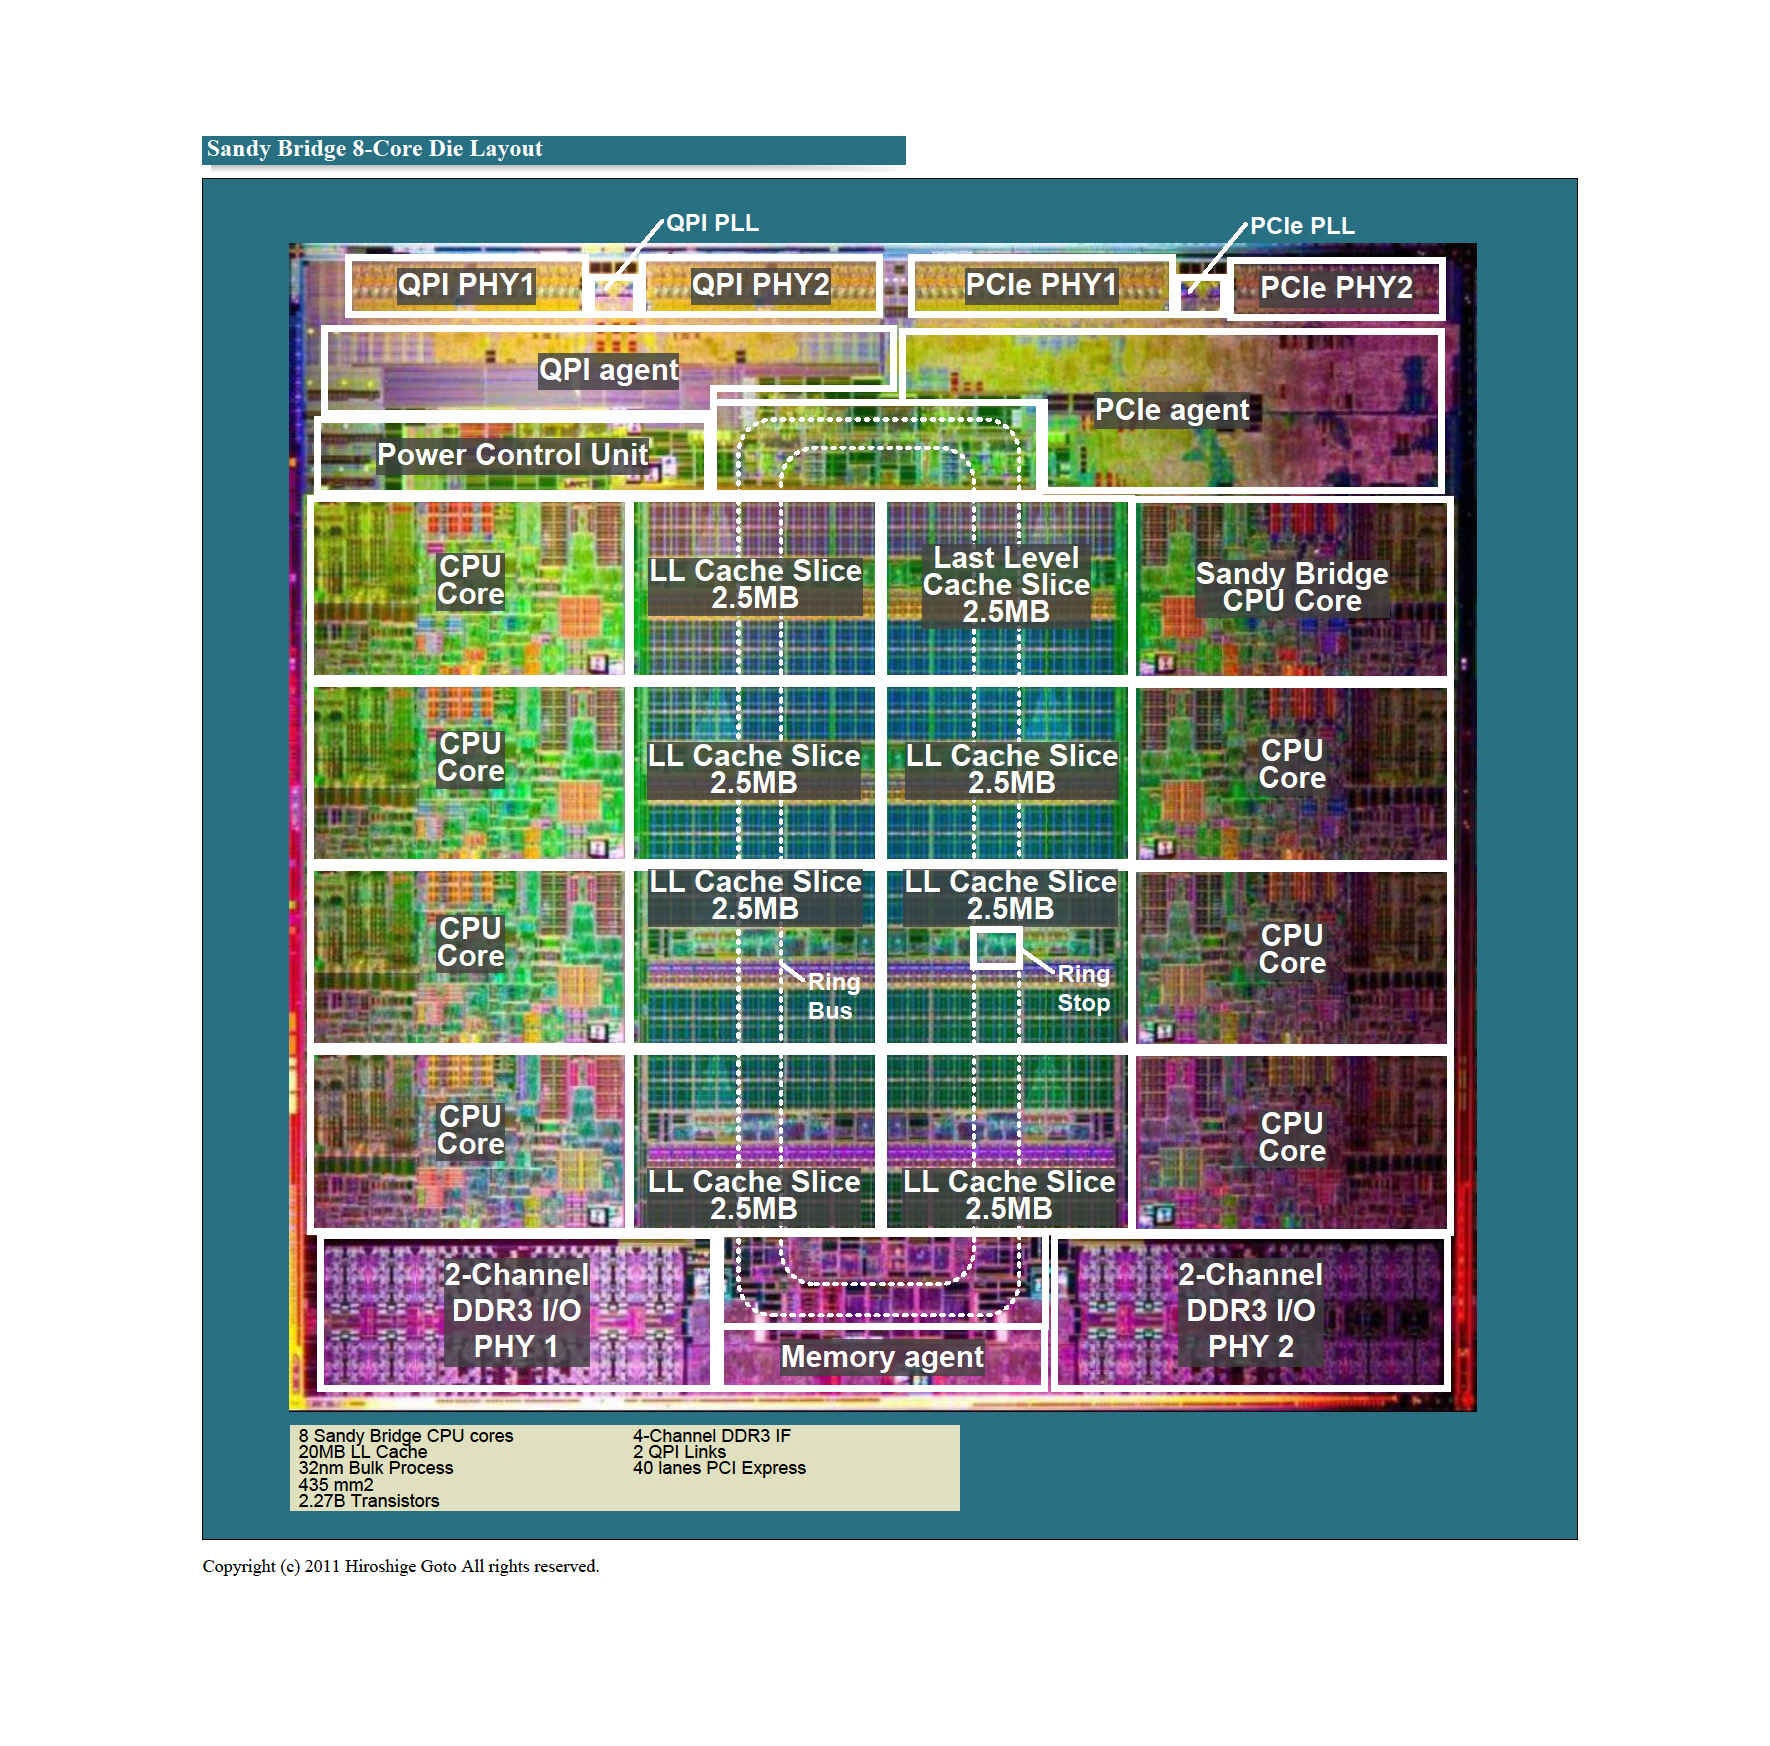
\includegraphics[scale=.13]{sandybridge-eightcore}
\end{frame}

\begin{frame}{Structure of a core}
  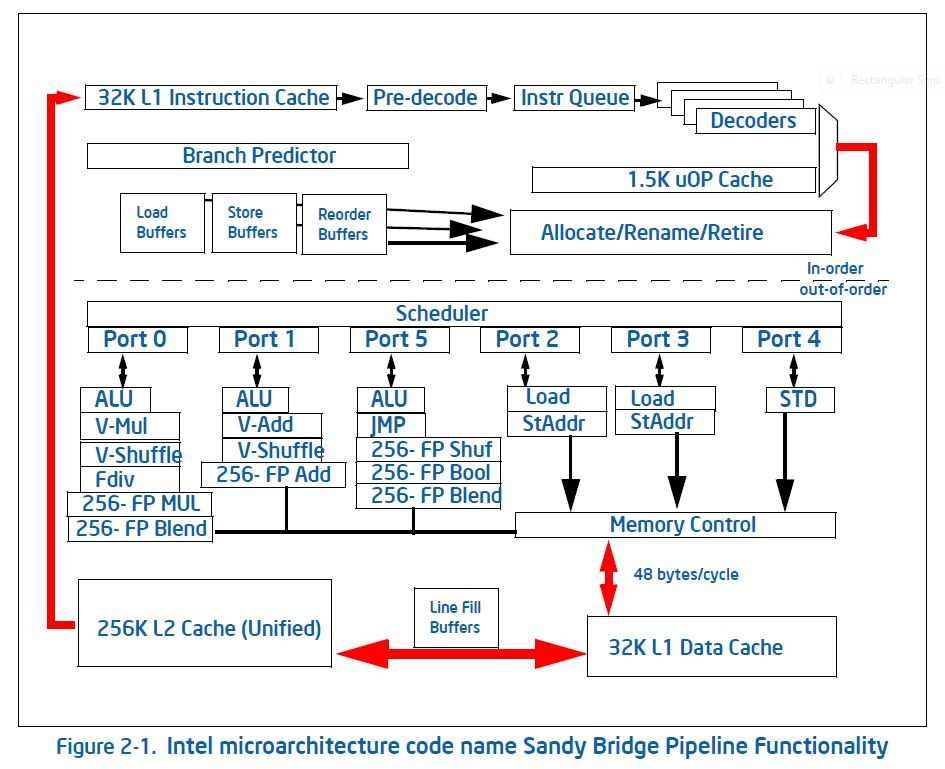
\includegraphics[scale=.4]{sandybridge_pipeline}
\end{frame}

\begin{frame}{Pipelining, pictorially}
    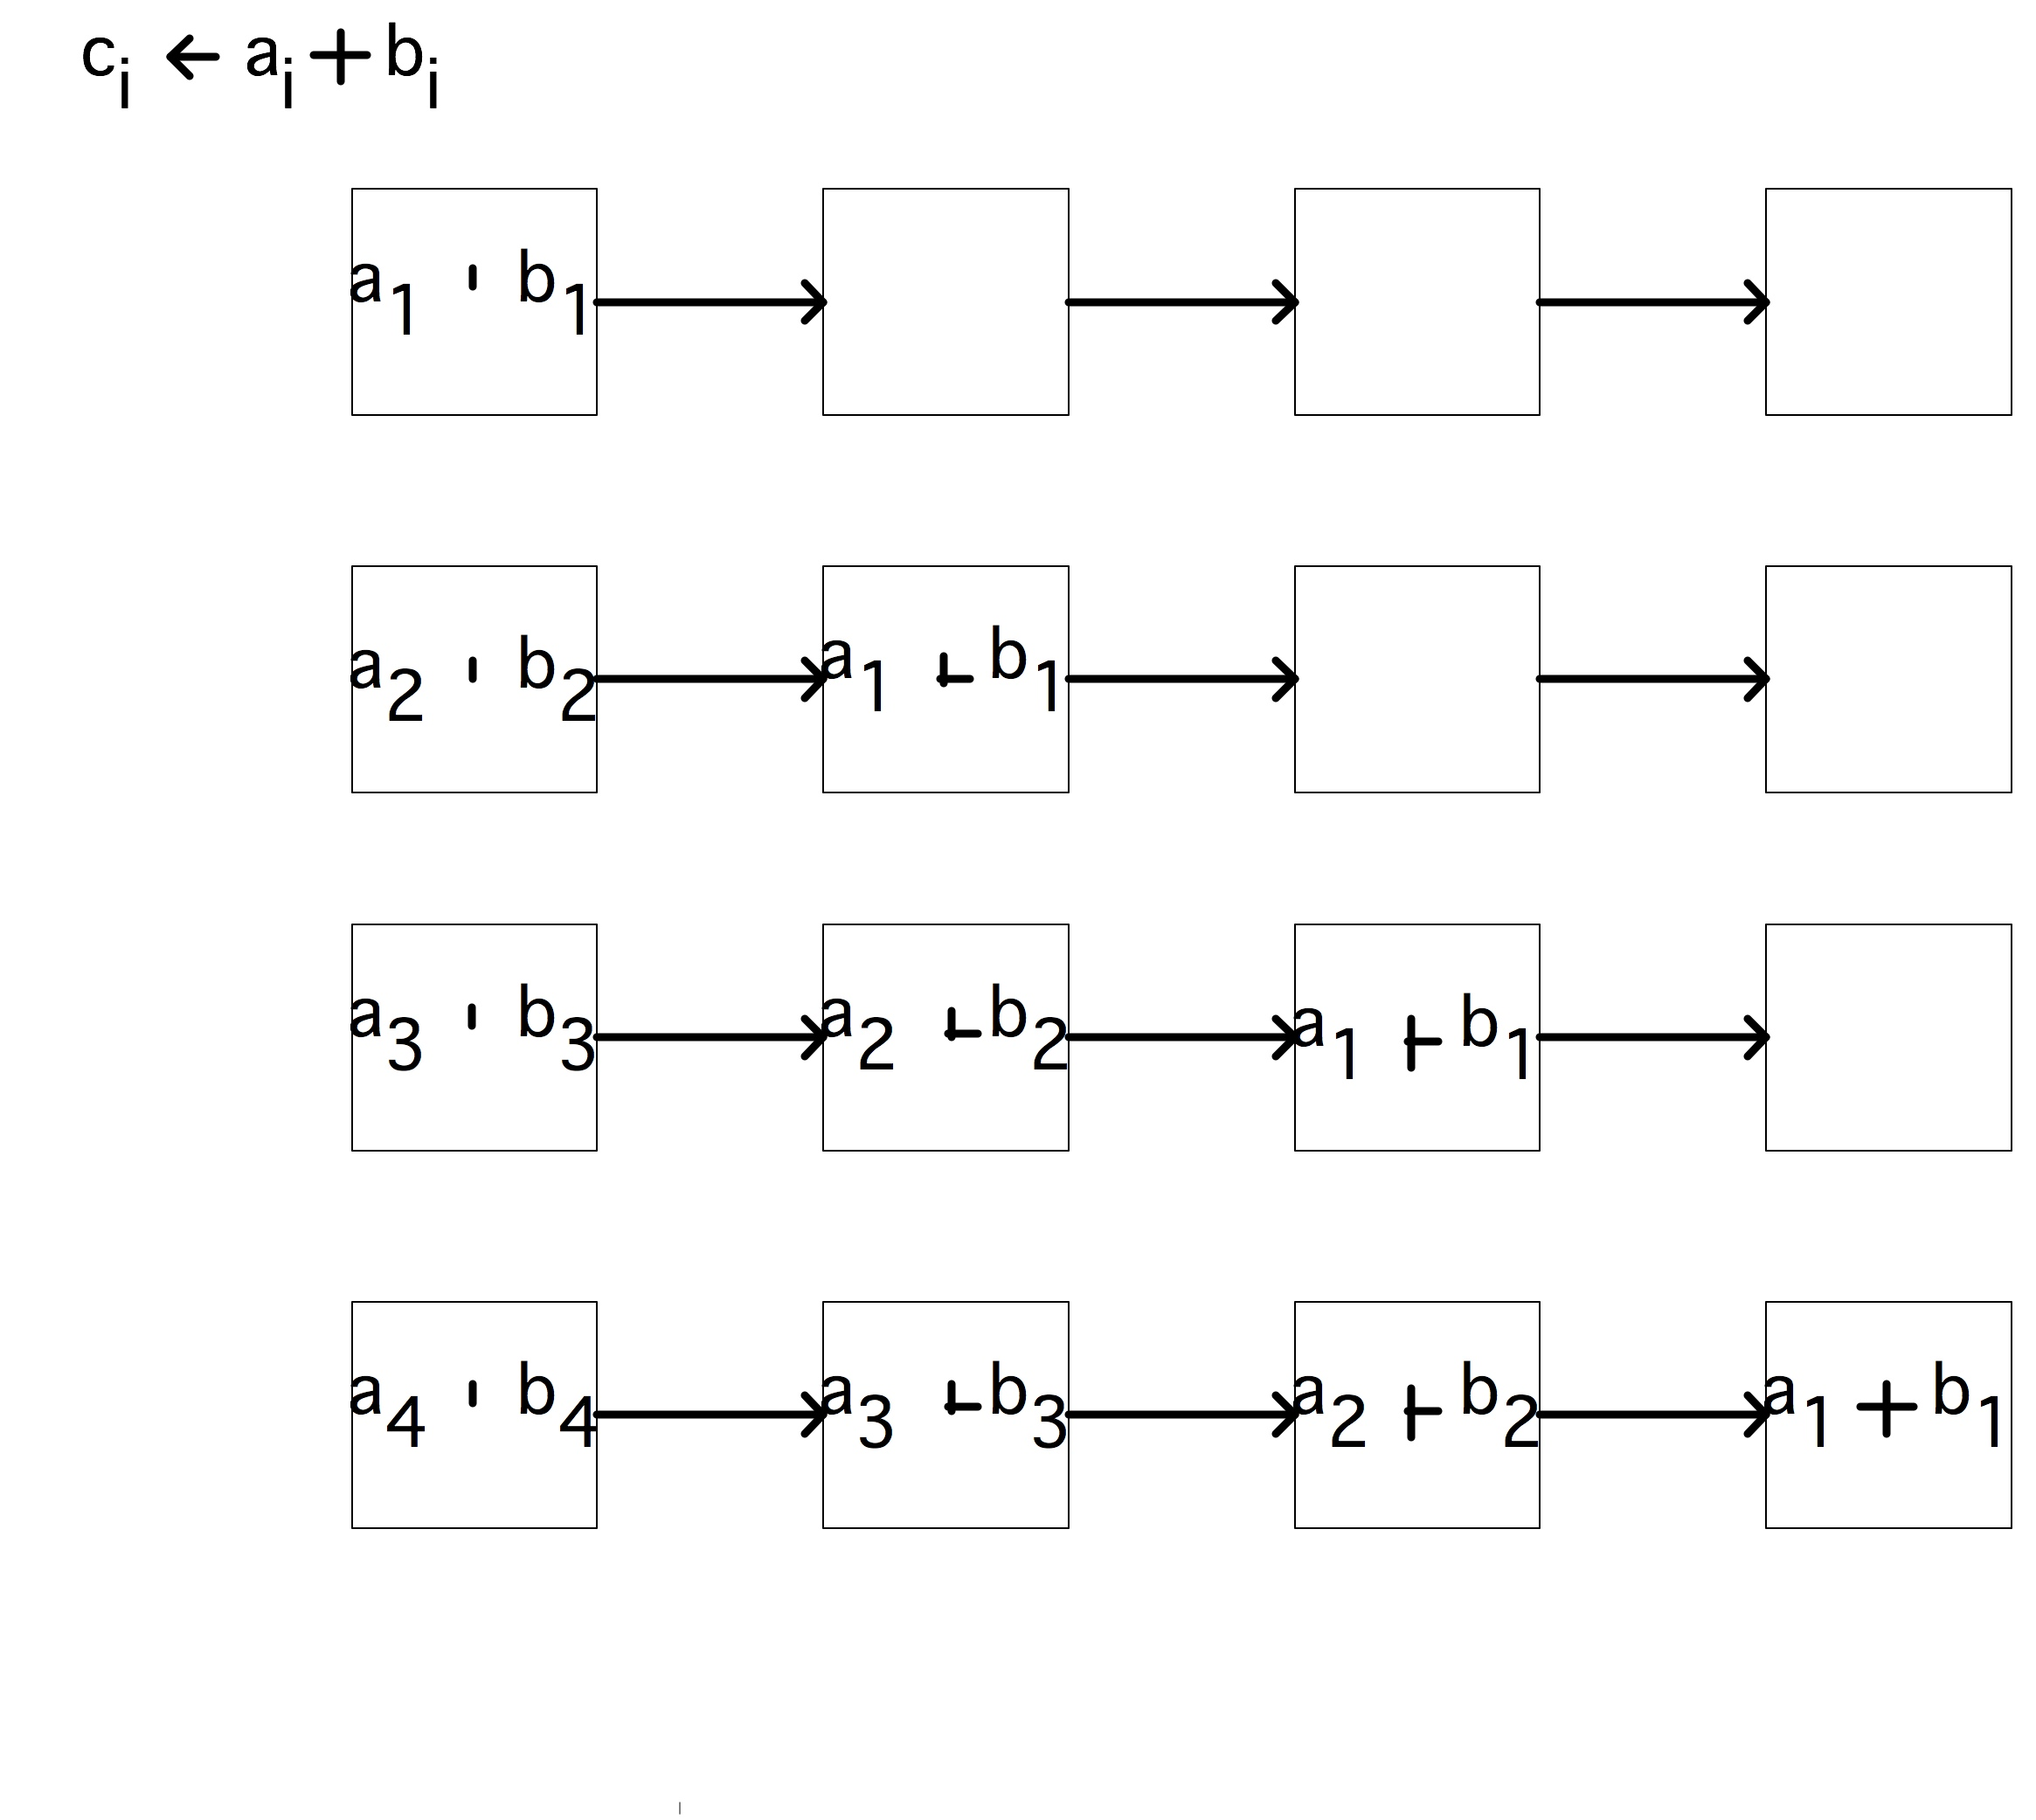
\includegraphics[scale=.1]{pipeline}
\end{frame}

\begin{frame}{Pipelining, formally}
  \begin{itemize}
\item Decoding the instruction  operands.
\item Data fetch into register
\item Aligning the exponents:
\[ 
\begin{array}{ll}
.35\times 10^{-1}\,+\, .6\times 10^{-2}&\hbox{becomes}\\
.35\times 10^{-1}\,+\, .06\times 10^{-1}.
\end{array}
\]
\item Adding mantissas, giving  $.41$.
\item Normalizing the result, giving $.41\times 10^{-1}$.
\item Storing the result.
\end{itemize}
\indextermbus{pipeline}{stages}
\end{frame}

\begin{frame}{Analysis}
Operation timing:
\[ 
\begin{cases}
  n&\hbox{operations}\\ \ell&\hbox{number of stages}\\ \tau&\hbox{clock cycle}
\end{cases} \Rightarrow
t(n)=n\ell\tau
\]
With pipelining:
\[ t(n)=[s+\ell+n-1]\tau \]
where $s$ is a setup cost

Asymptotic speedup is $\ell$

$n_{1/2}$: value for which speedup is $\ell/2$
\end{frame}

\begin{frame}[fragile]{Applicability of pipelining}
  Pipelining works for:\\
  vector addition

Pipelining does not work for:\\
recurrences
\begin{verbatim}
for (i) {
  x[i+1] = a[i]*x[i] + b[i];
}
\end{verbatim}
Transform:
\[
\begin{array}{rl}
  x_{n+2}=&a_{n+1}x_{n+1}+b_{n+1}\\
    &=a_{n+1}(a_nx_n+b_n)+b_{n+1}\\
    &=a_{n+1}a_nx_n + a_{n+1}b_n+b_{n+1}
\end{array}
\]
\end{frame}

\begin{frame}{Instruction pipeline}
  \begin{itemize}
  \item Instruction-Level Parallelism: more general notion of 
    independent instructions
  \item Requires independent instructions
  \item As frequency goes up, pipeline gets longer: more demands on compiler
  \end{itemize}
\end{frame}

\begin{frame}{Instruction-Level Parallelism}
  \begin{itemize}
  \item multiple-issue of independent instructions
  \item branch prediction and speculative execution
  \item out-of-order execution
  \item prefetching
  \end{itemize}
  Problems: complicated circuitry, hard to maintain performance
\end{frame}

\begin{frame}{Implications}
  \begin{itemize}
  \item Long pipeline needs many independent instructions:\\
    demands on compiler
  \item Conditionals break the stream of independent instructions
    \begin{itemize}
    \item Processor tries to predict branches
    \item \indexterm{branch misprediction penalty}:\\
      pipeline needs to be flushed and refilled
    \item avoid conditionals in inner loops!
    \end{itemize}
  \end{itemize}
\end{frame}

\begin{frame}{Peak performance}
\small
Performance is a function of
\begin{itemize}
\item Clock frequency,
\item SIMD width
\item Load/store unit behaviour
\end{itemize}
Behaviour (out of L1):

  \begin{tabular}{lllll}
Processor&year&add/mult/fma units  &daxpy cycles\\
         &    &(count$\times$width)&(arith vs load/store)\\
\toprule
MIPS R10000       &1996 &$1\times1+1\times1+0$ &8/24 \\
Alpha EV5         &1996 &$1\times1+1\times1+0$ &8/12 \\
IBM Power5        &2004 &$0+0+2\times1       $ &4/12 \\
AMD Bulldozer     &2011 &$2\times2+2\times2+0$ &2/4  \\
Intel Sandy Bridge&2012 &$1\times4+1\times4+0$ &2/4  \\
Intel Haswell     &2014 &$0+0+2\times 4      $ &1/2  \\
%Intel Woodcrest, AMD Barcelona&2 add + 2 mul&4 \\  %SIMD FADD, FMUL
%IBM POWER4, POWER5, POWER6&    2 FMA & 4 \\
%IBM BG/L, BG/P & 1 SIMD FMA & 4 \\
%SPARC IV & 1 add + 1 mul& 2 \\
%Itanium2 &  2 FMA & 4 
  \end{tabular}

Floating point capabilities of several processor architectures,
  and DAXPY cycle number for 8 operands  
\end{frame}

\begin{frame}{Dirty secret}
  Processor design is sometimes optimized for certain algorithms

  In particular: DGEMM/Linpack

  Favourable property: one load per operation, no stores
\end{frame}

\Level 1 {Memory hierarchy: caches, register, TLB.}

\begin{frame}{The Big Story}
  \begin{itemize}
  \item DRAM memory is slow, so let's put small SRAM close to the processor
  \item This helps if data is reused 
  \item Does the algorithm have reuse?
  \item Does the implementation reuse data?
  \end{itemize}
\end{frame}

\begin{frame}{Bandwidth and latency}
  Important theoretical concept:
  \begin{itemize}
  \item \indexterm{latency} is delay between request for data and availability
  \item \indexterm{bandwidth} is rate at which data arrives thereafter
  \end{itemize}
\end{frame}

\begin{frame}
  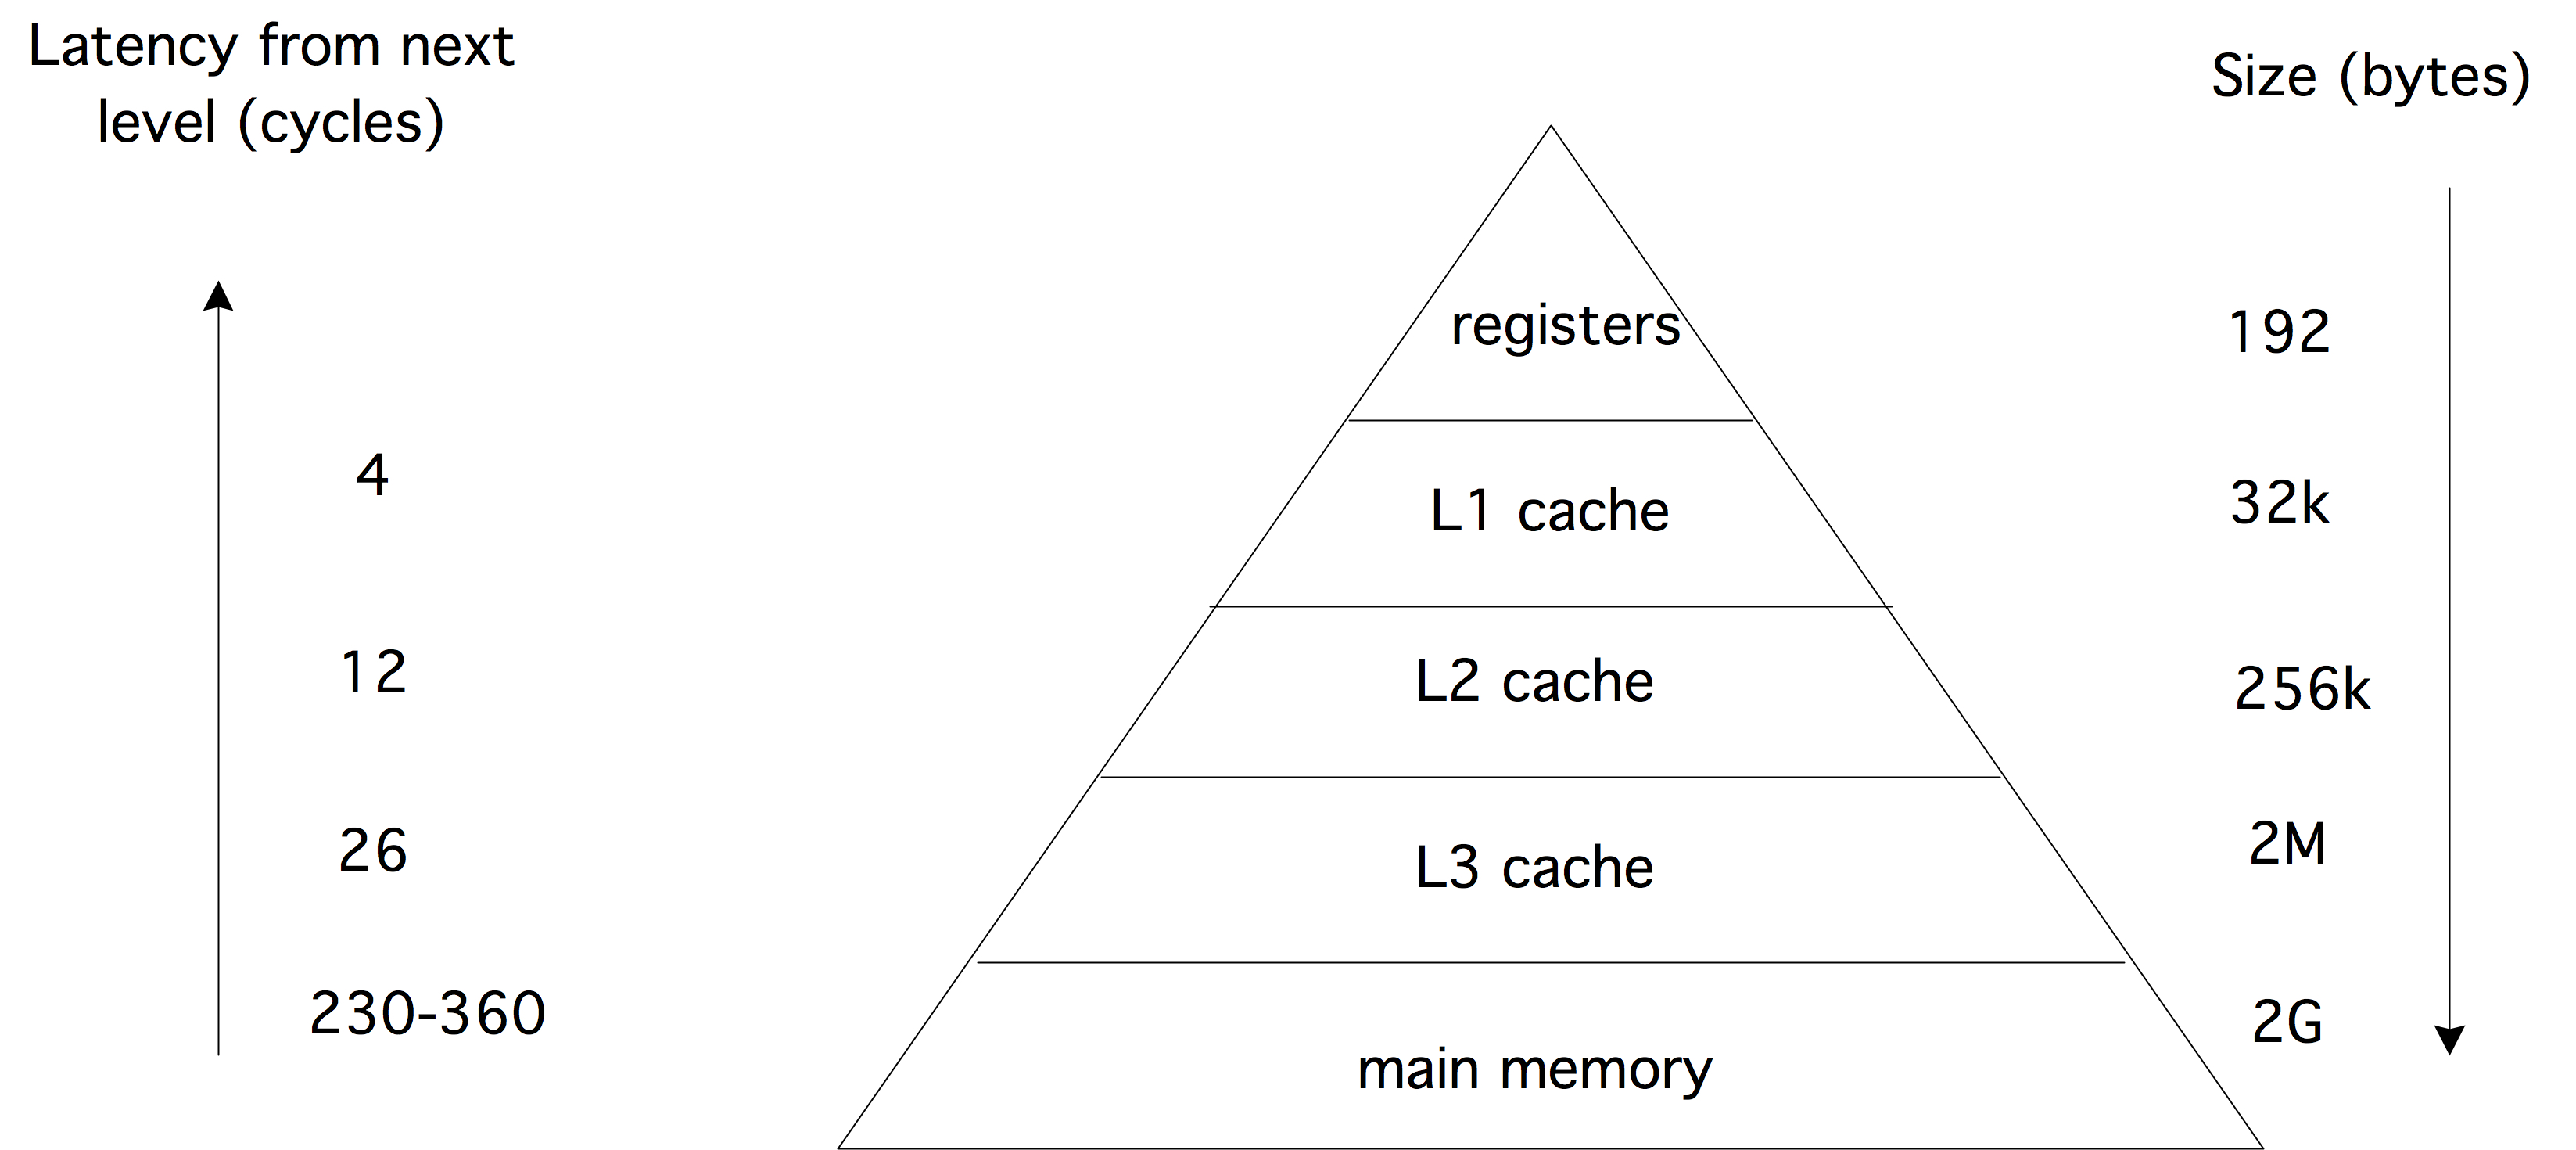
\includegraphics[scale=.1]{hierarchysb}  
\end{frame}

\Level 2 {Registers}

\begin{frame}[fragile]{Computing out of registers}
\begin{verbatim}
a := b + c
\end{verbatim}
\begin{itemize}
\item load the value of \n{b} from memory into a \indexterm{register},
\item load the value of \n{c} from memory into another register,
\item compute the sum and write that into yet another register, and
\item write the sum value back to the memory location of~\n{a}.
\end{itemize}
\end{frame}

\begin{frame}[fragile]{Register usage}
Assembly code
\begin{verbatim}
addl	%eax, %edx
\end{verbatim}  
\begin{itemize}
\item Registers are named
\item Can be explicitly addressed by the programmer
\item \ldots as opposed to caches.
\item Assembly coding or inline assembly (compiler dependent)
\item \ldots but typically generated by compiler
\item Very high bandwidth / low latency: peak performance only possible with
data in register.
\end{itemize}
\end{frame}

\begin{frame}[fragile]{Examples of register usage}

\begin{verbatim}
a := b + c
d := a + e
\end{verbatim}
\n{a} stays resident in register, avoid store and load  

\begin{verbatim}
t1 = sin(alpha) * x + cos(alpha) * y;
t2 = -cos(alpha) * x + sin(alpha) * y;
\end{verbatim}
subexpression elimination:
\begin{verbatim}
s = sin(alpha); c = cos(alpha);
t1 = s * x + c * y;
t2 = -c * x + s * y
\end{verbatim}
often done by compiler
\end{frame}

\begin{frame}[fragile]{Register variables}
Hint to the compiler: declare \indextermbus{register}{variable}
\begin{verbatim}
register double t;
\end{verbatim}
Declaring too many leads to register spill.
\end{frame}

\Level 2 {Caches}

\begin{frame}[fragile]{Cache basics}
Fast SRAM in between memory and registers: mostly serves data reuse
\begin{verbatim}
... = ... x ..... // instruction using x
.........         // several instructions not involving x
... = ... x ..... // instruction using x
\end{verbatim}
\begin{itemize}
\item load \n{x} from memory into cache, and from cache into register;
  operate on it;
\item do the intervening instructions;
\item request \n{x} from memory, but since it is still in the cache,
  load it from the cache into register; operate on it.
\item essential concept: \indexterm{data reuse}
\end{itemize}
Caches are associative
\end{frame}

\begin{frame}{Cache levels}
  \index{cache!levels}
  \begin{itemize}
  \item Levels 1,2,3(,4): L1, L2, etc.
  \item Increasing size, increasing latency, increasing bandwidth
  \item (Note: L3/L4 can be fairly big; beware benchmarking)
  \item Cache hit / cache miss: one level is consulted, then the next
  \item L1 has separate data / instruction cache, other levels mixed
  \item Caches do not have enough bandwidth to serve the processor:
    coding for reuse on all levels.
  \end{itemize}
\end{frame}

\begin{frame}{Cache misses}
  \index{cache!miss}
  \begin{itemize}
  \item Compulsory miss: first time data is referenced
  \item Capacity miss: data was in cache, but has been flushed (overwritten)
    by LRU policy
  \item Conflict miss: two items get mapped to the same cache location,
    even if there are no capacity problems
  \item Invalidation miss: data becomes invalid because of activity of another core
  \end{itemize}  
\end{frame}

\begin{frame}[fragile]{Illustration of capacity}
\small
\begin{verbatim}
for (i=0; i<NRUNS; i++)
  for (j=0; j<size; j++)
    array[j] = 2.3*array[j]+1.2;
\end{verbatim}
  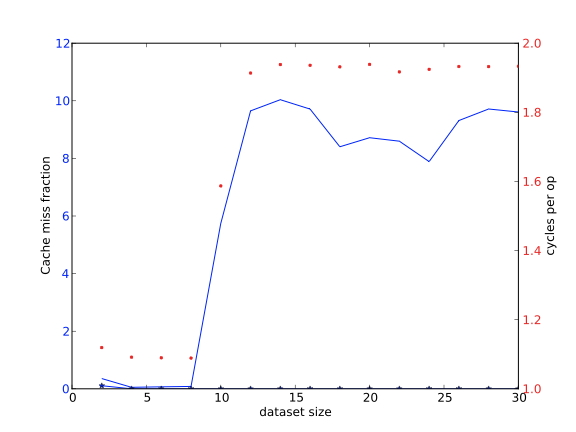
\includegraphics[scale=.4]{cacheoverflow}
\end{frame}

\begin{frame}{Cache lines}
  \begin{itemize}
  \item Memory requests go by byte or word
  \item Memory transfers go by \indextermbus{cache}{line}:\\ 4~or~8 words
  \item Cache line transfer costs bandwidth
  \item $\Rightarrow$ important to use all elements
  \end{itemize}
\end{frame}

\begin{frame}[fragile]{Cache line use}
\begin{verbatim}
for (i=0; i<N; i++)
  ... = ... x[i] ...
\end{verbatim}
  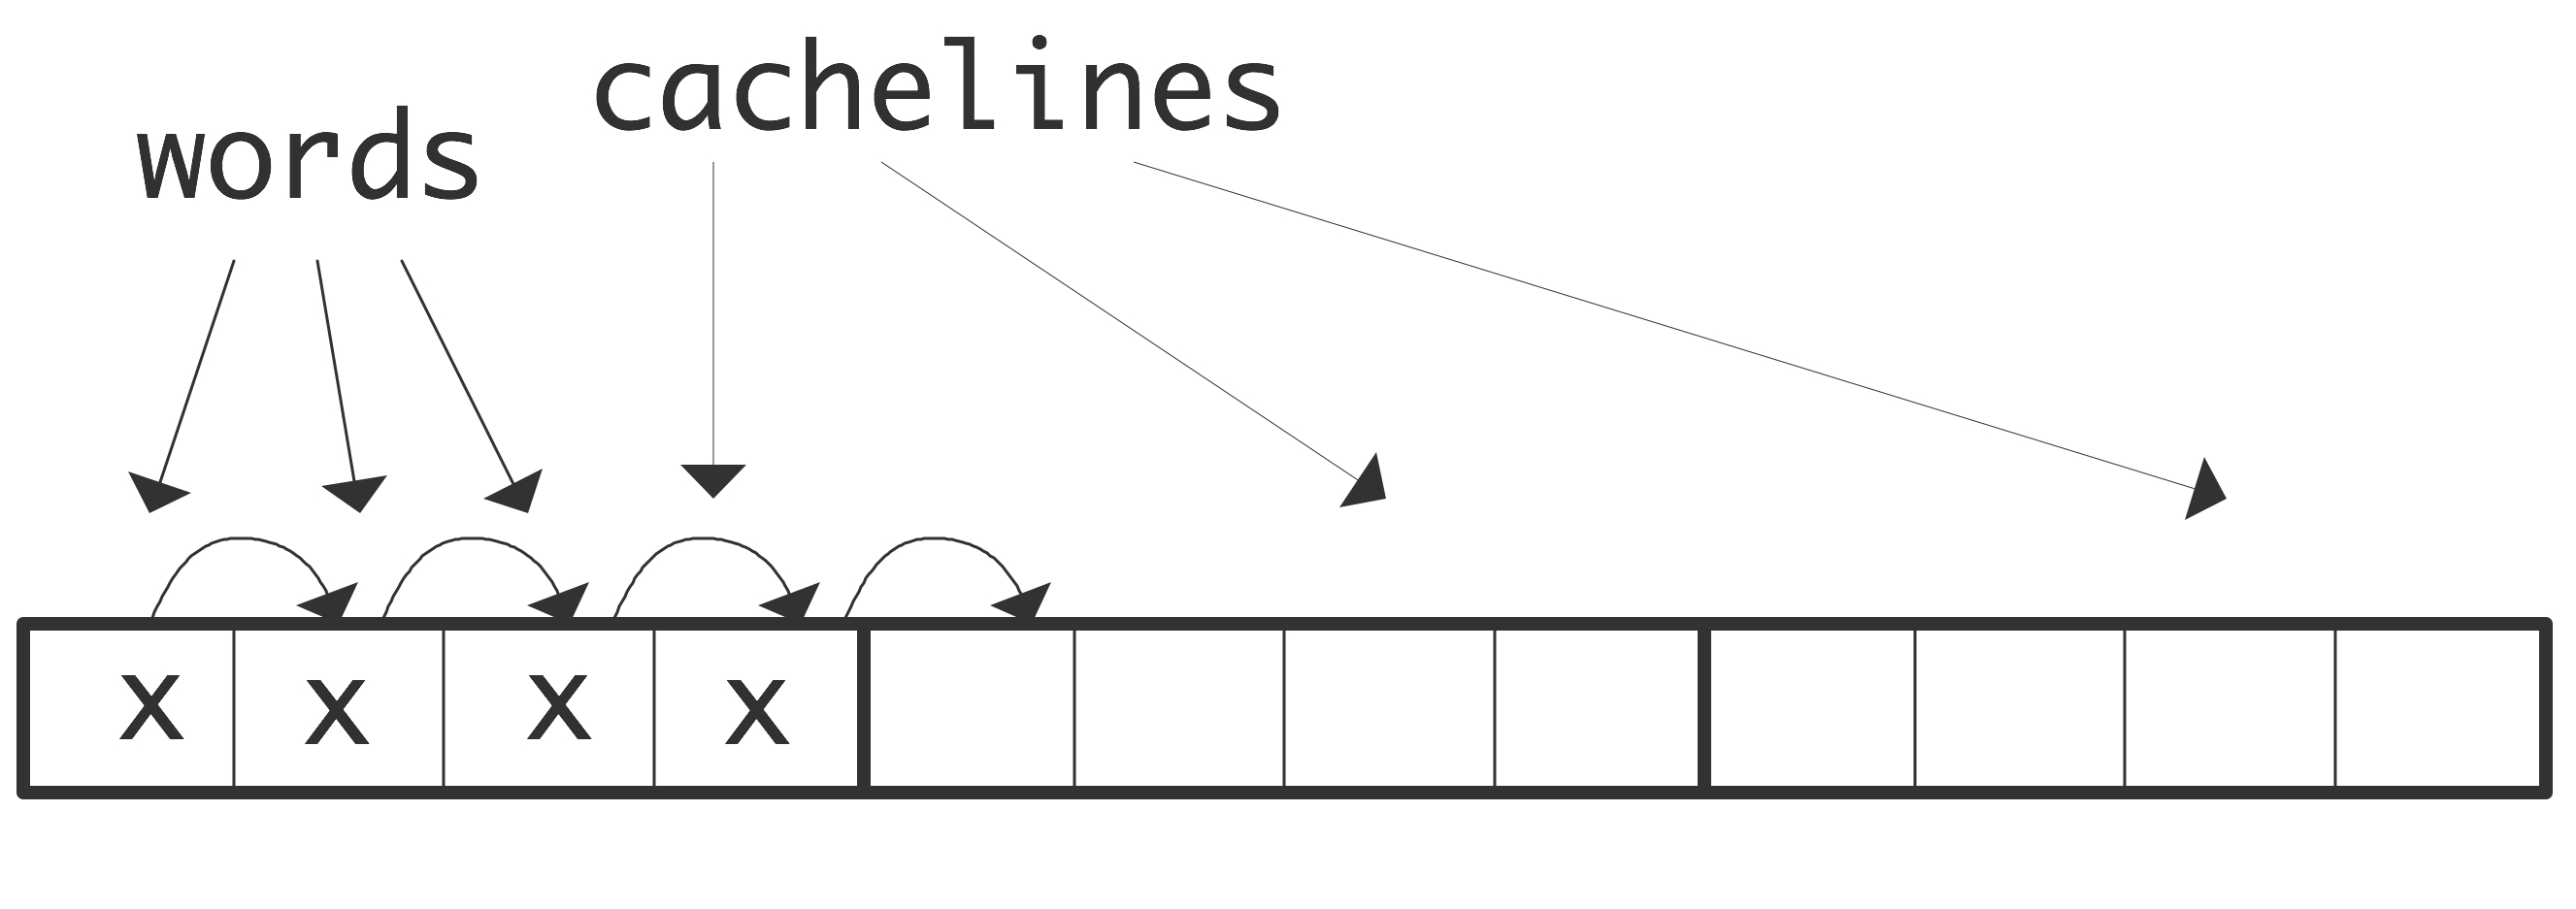
\includegraphics[scale=.07]{stride-1}
\begin{verbatim}
for (i=0; i<N; i+=stride)
  ... = ... x[i] ...
\end{verbatim}
  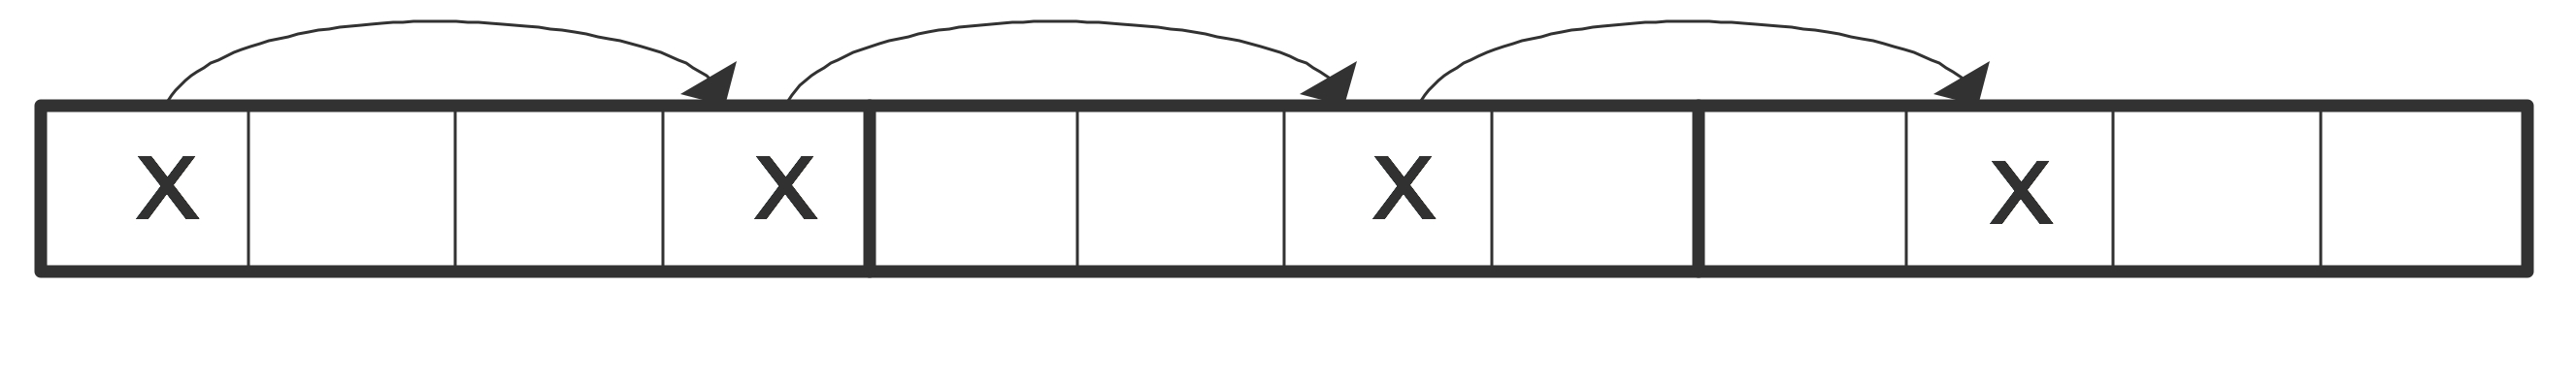
\includegraphics[scale=.07]{stride-3}
\end{frame}

\begin{frame}[fragile]{Stride effects}
\small
\begin{verbatim}
for (i=0,n=0; i<L1WORDS; i++,n+=stride)
  array[n] = 2.3*array[n]+1.2;
\end{verbatim}
  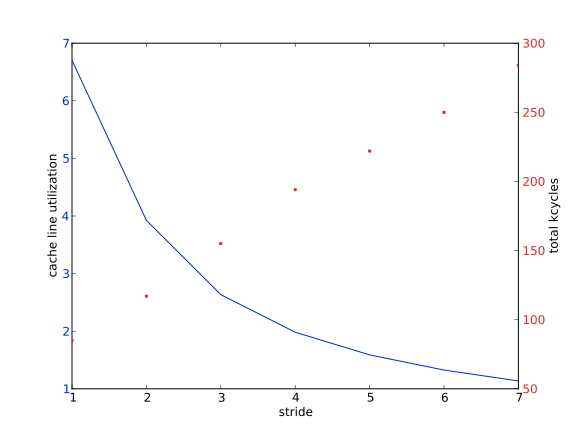
\includegraphics[scale=.4]{cacheline8}
\end{frame}

\begin{frame}{Spatial and temporal locality}
  Temporal locality: use an item, use it again but from cache\\
  efficient because second transfer cheaper.

  Spatial locality: use an item, then use one `close to it'\\
  (for instance from same cacheline)\\
  efficient because item is already reachable even though not used before.
\end{frame}

\begin{frame}{Cache mapping}
  Cache is smaller than memory, so we need a mapping scheme
  \begin{itemize}
  \item Ideal: any address can go anywhere; LRU policy for replacement
  \item pro: optimal; con: slow, expensive to manufacture
  \item Simple: direct mapping by truncating addresses
  \item pro: fast and cheap; con: I'll show you in a minute
  \item Practical: limited associativity; golden mean
  \end{itemize}
\end{frame}

\begin{frame}{Direct mapping}
  \index{cache!direct mapping}
  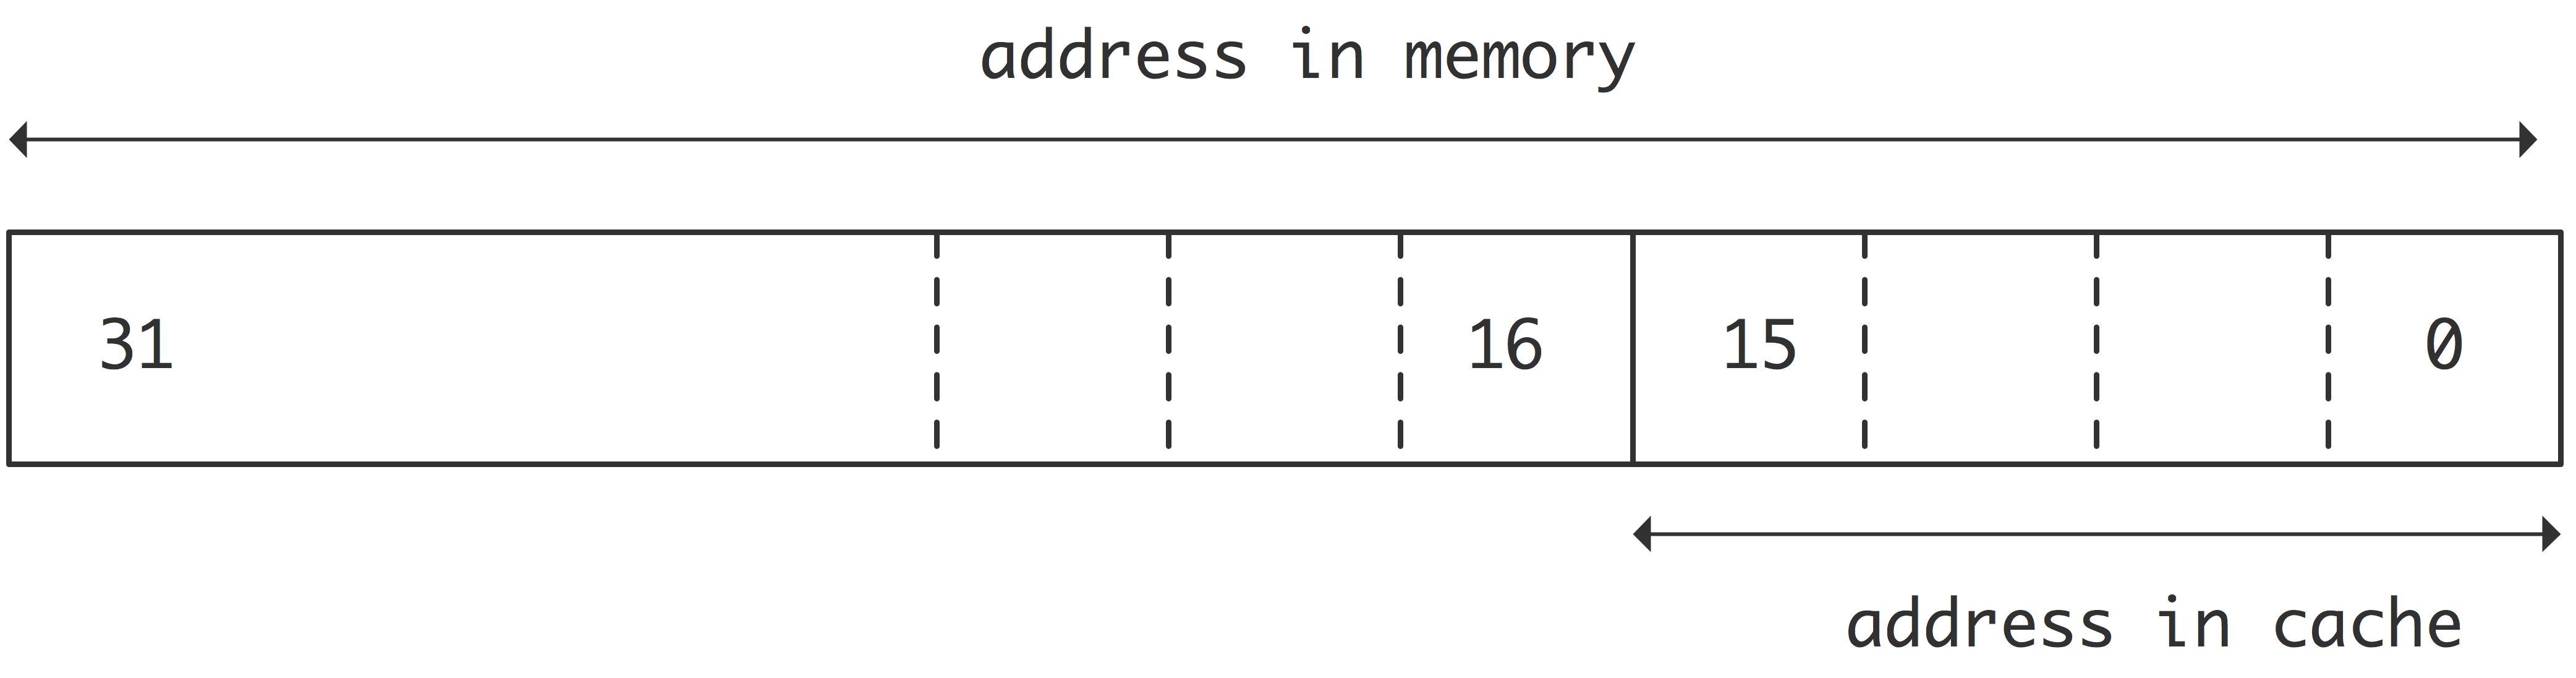
\includegraphics[scale=.06]{directmap}

Direct mapping of 32-bit addresses into a 64K cache
\begin{itemize}
\item Use last number of bits to find cache address
\item If (memory) addresses are cache size apart, they get mapped
  to the same cache location
\item If you traverse an array, a contiguous chunk will be mapped
  to cache without conflict.
\end{itemize}
\end{frame}

\begin{frame}[fragile]{The problem with direct mapping}
\begin{verbatim}
real*8 A(8192,3);
do i=1,512
  a(i,3) = ( a(i,1)+a(i,2) )/2
end do
\end{verbatim}
In each iteration 3 elements map to the same cache location:\\
constant overwriting (`eviction', \indextermbus{cache}{thrasing}):\\
low performance
\end{frame}

\begin{frame}{Associate cache mapping}  
  \index{cache!associative mapping}
  \begin{itemize}
  \item Allow each memory address to go to multiple (but not all) cache addresses;
    typically 2,4,8
  \item Prevents problems with multiple arrays
  \item Reasonable fast, still:
  \item Often lower associativity for L1 than L2, L3
  \end{itemize}
  \begin{tabular}{|l|ll|}
    \toprule
    Associativity&L1&L2\\
    \midrule
    Intel (Woodcrest)&8&8\\
    AMD (Bulldozer)&2&8\\
    \bottomrule
  \end{tabular}
\end{frame}

\begin{frame}{Illustration of associativity}
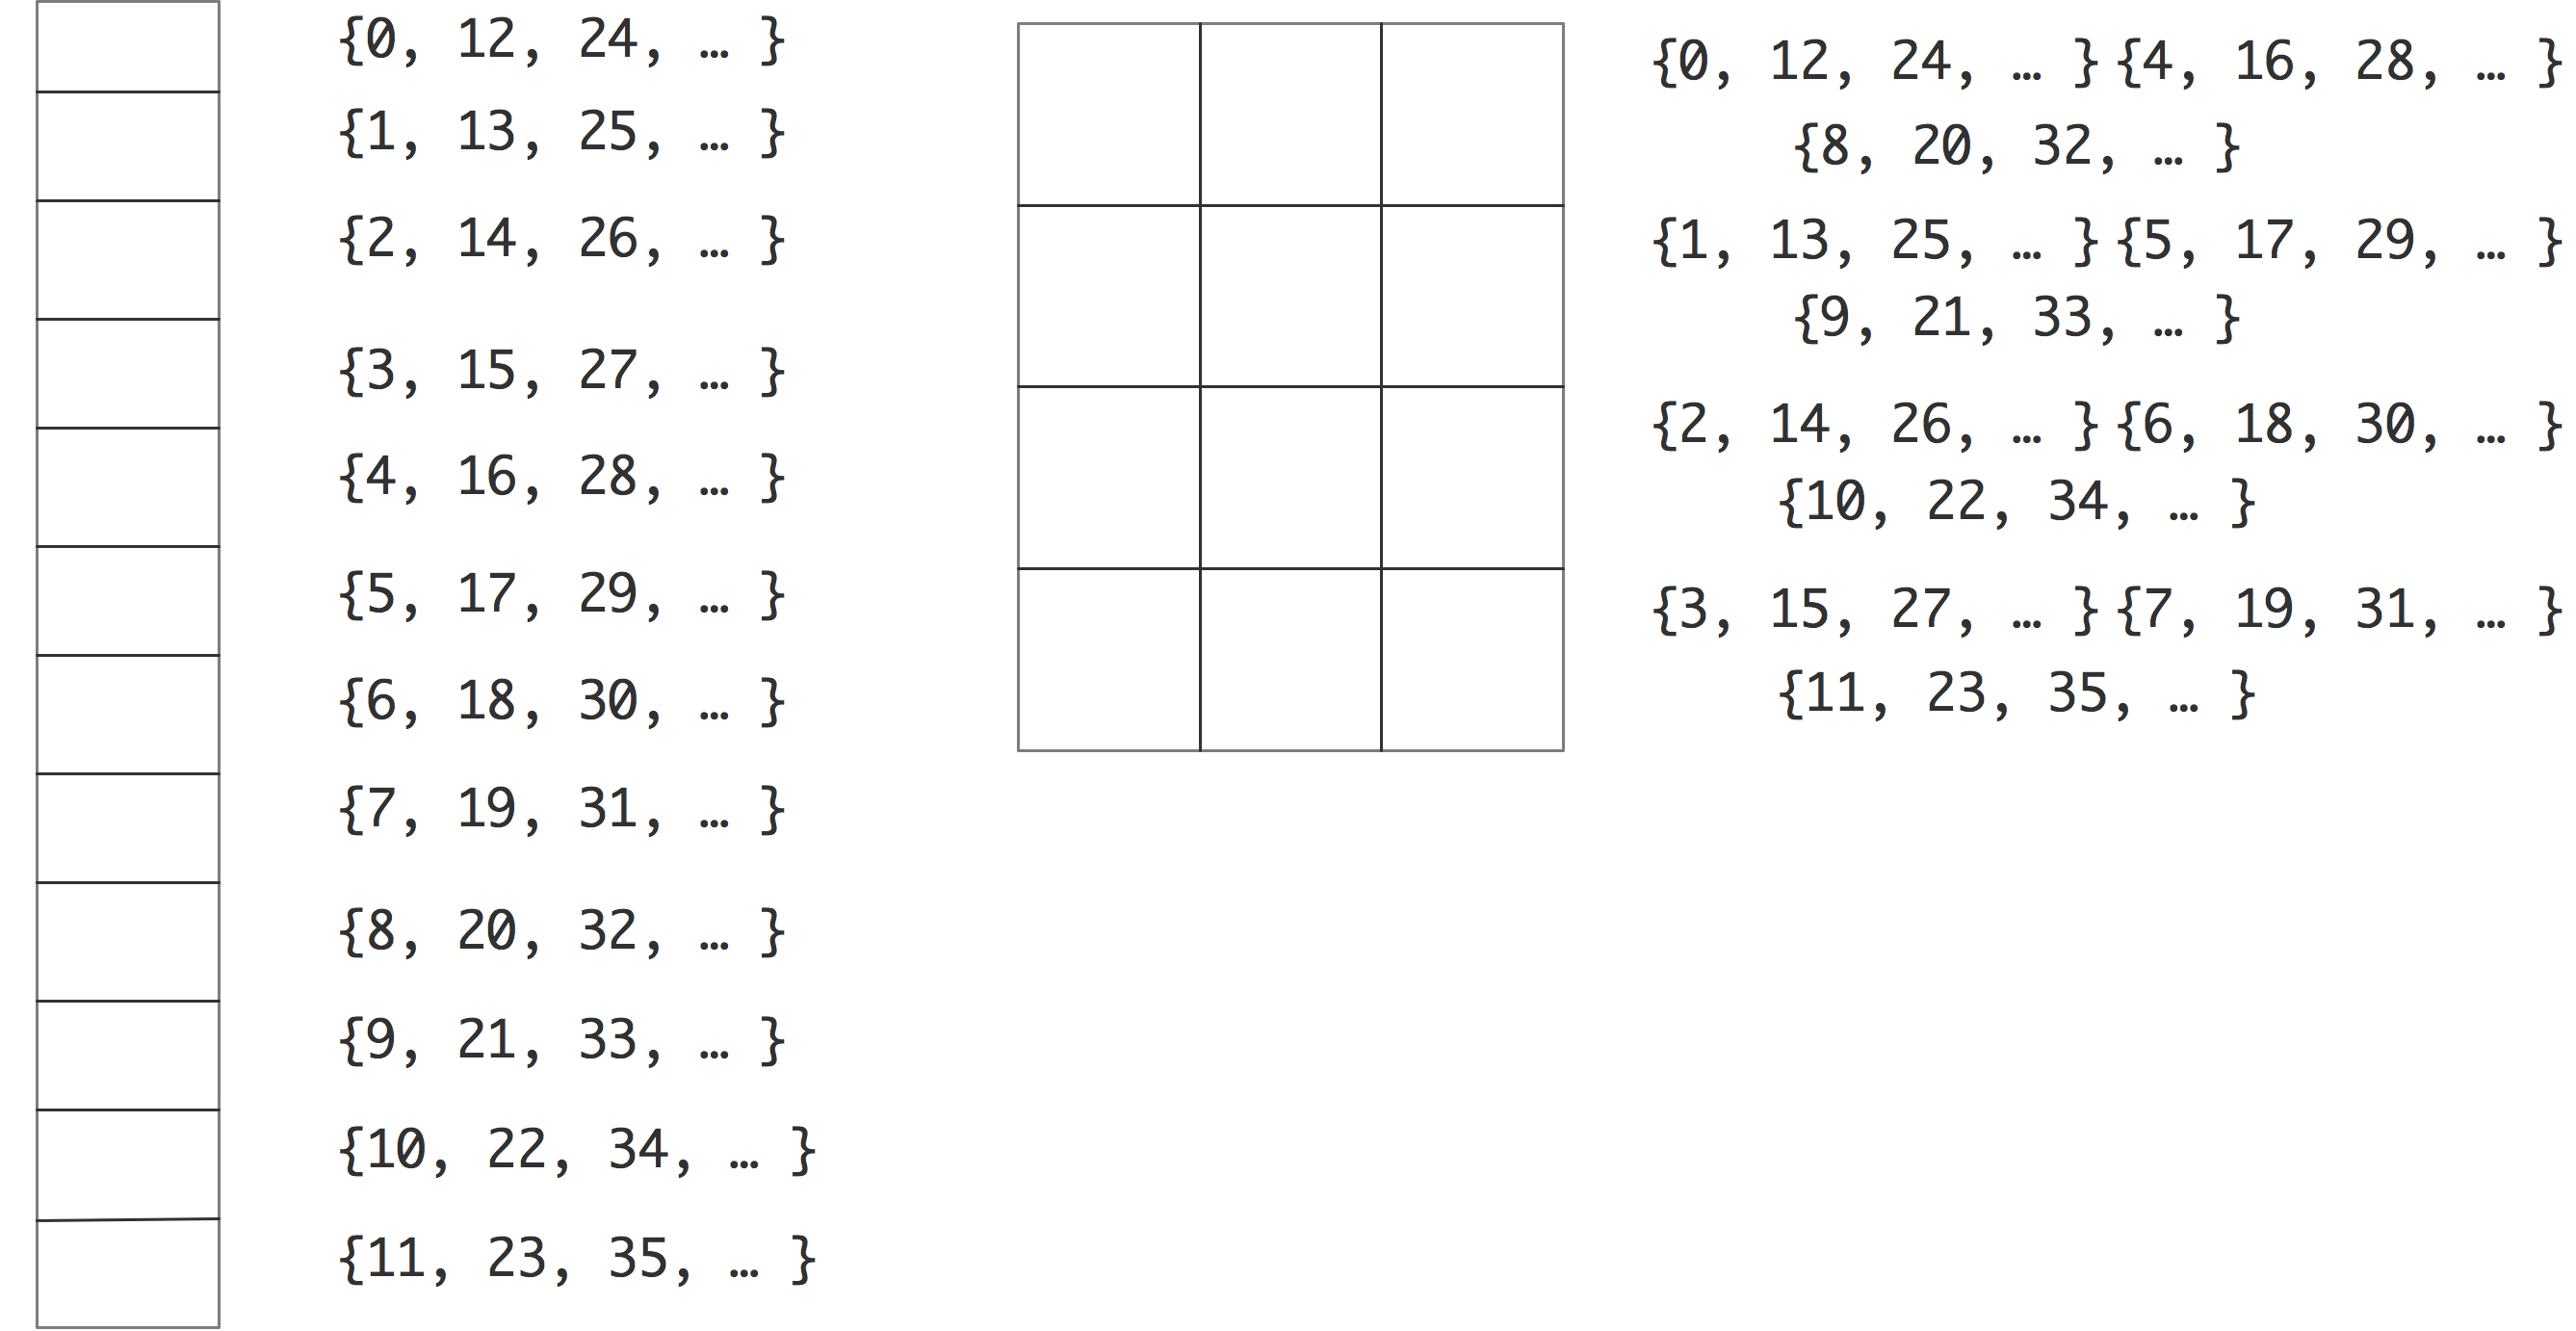
\includegraphics[scale=.1]{assoc-mapping}

Two caches of 12 elements: direct mapped (left) and 3-way associative (right)

Direct map: 0--12 is conflict\\ Associative: no conflict
\end{frame}

\begin{frame}{Associativity in practice}
\[ \forall_j\colon y_j= y_j+\sum_{i=1}^mx_{i,j} \]
  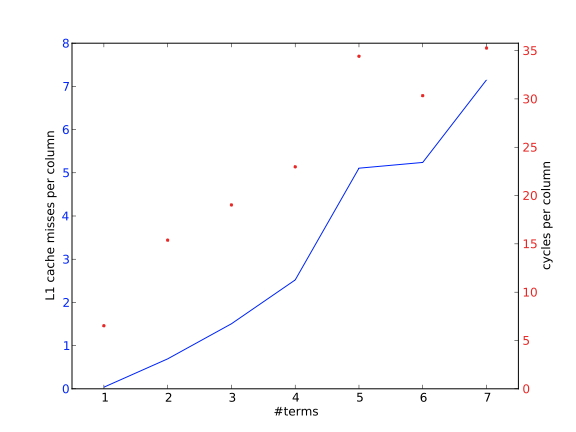
\includegraphics[scale=.4]{l1_assoc}

The number of L1 cache misses and the number of cycles for
    each $j$ column accumulation, vector length~$4096$
\end{frame}

\begin{frame}{One remedy}
Do not user powers of 2.

  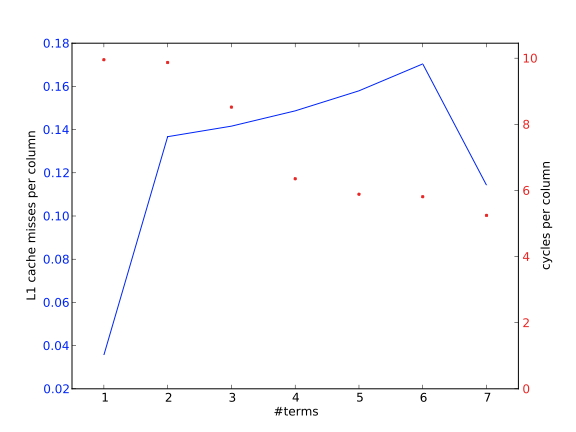
\includegraphics[scale=.4]{l1_assocshift}

The number of L1 cache misses and the number of cycles for
    each $j$ column accumulation, vector length~$4096+8$
\end{frame}

\Level 2 {More memory system topics}

\begin{frame}{Bandwidth / latency}
  Simple model for sending $n$ words: \[ t=\alpha + \beta n \]
  Quoted bandwidth figures are always optimistic:
  \begin{itemize}
  \item bandwidth shared between cores
  \item bandwidth wasted on coherence
  \item assumes optimal scheduling of DRAM banks
  \end{itemize}
\end{frame}

\begin{frame}{Prefetch}
  \begin{itemize}
  \item Do you have to wait for every item from memory?
  \item Memory controller can infer streams: prefetch
  \item Sometimes controllable through assembly, directives, libraries (AltiVec)
  \item One form of latency hiding
  \end{itemize}
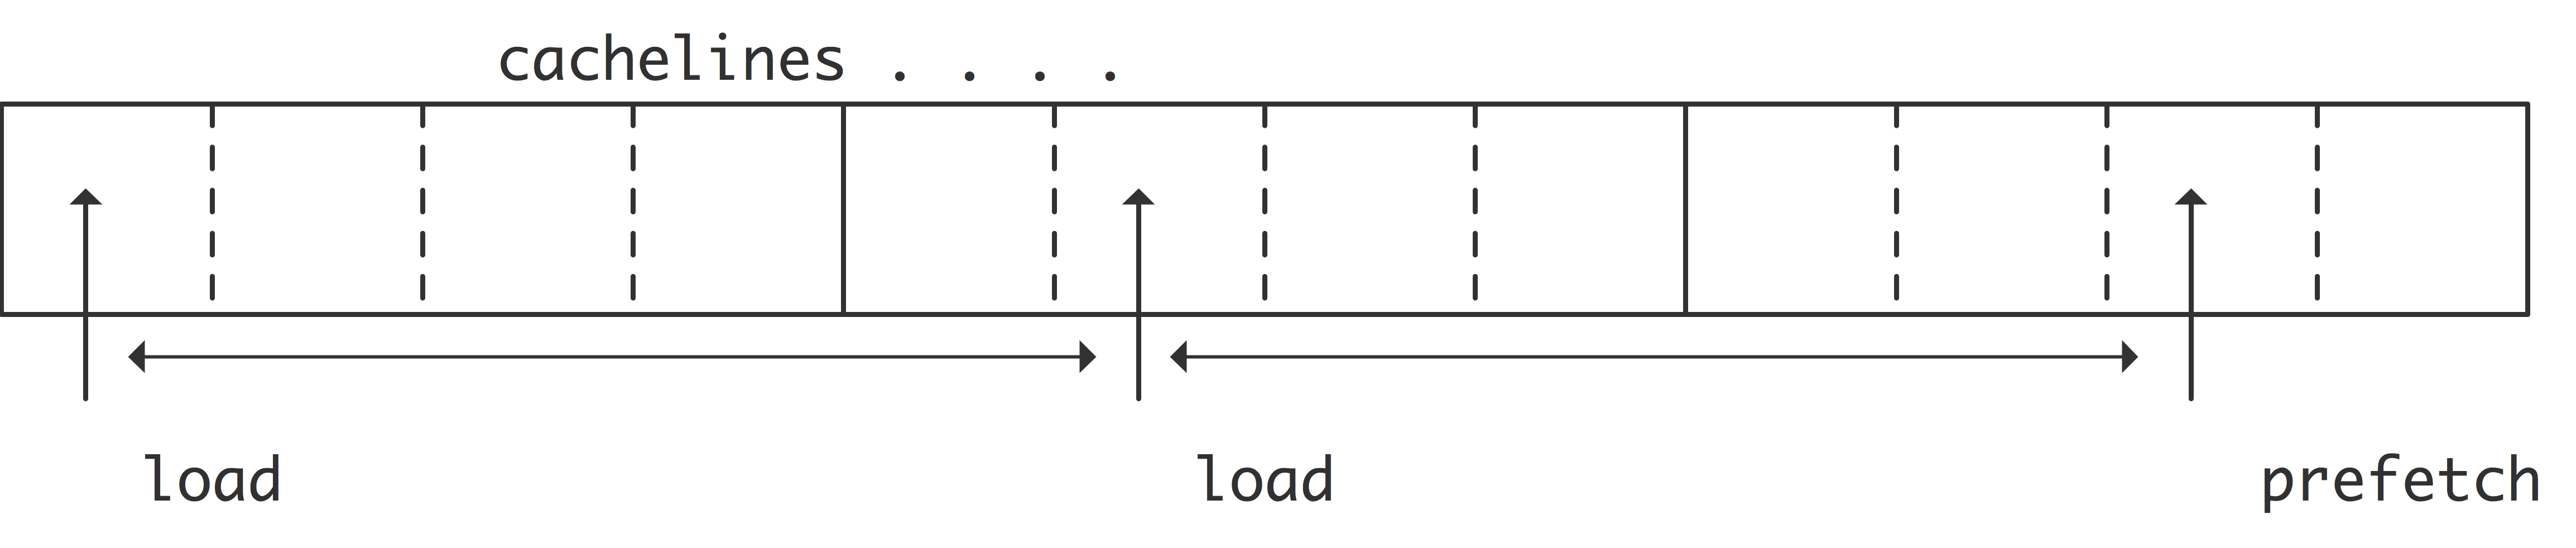
\includegraphics[scale=.06]{prefetch}
\end{frame}

\begin{frame}{Memory pages}
  Memory is organized in pages:
  \begin{itemize}
  \item Translation between logical address, as used by program,
    and physical in memory
  \item This serves virtual memory and relocatable code
  \item so we need another translation stage.
  \end{itemize}
\end{frame}

\begin{frame}{Page translation: TLB}
  \begin{itemize}
  \item General page translation: slowish but extensive
  \item \indexac{TLB} is a small list of frequently used pages
  \item Example of spatial locality: items on an already referenced page
    are found faster
  \end{itemize}
\end{frame}

\begin{frame}[fragile]{TLB misses}
\small
\begin{verbatim}
#define INDEX(i,j,m,n) i+j*m
array = (double*) malloc(m*n*sizeof(double));
/* traversal #2 */
for (i=0; i<m; i++)
  for (j=0; j<n; j++)
    array[INDEX(i,j,m,n)] = array[INDEX(i,j,m,n)]+1;
\end{verbatim}
  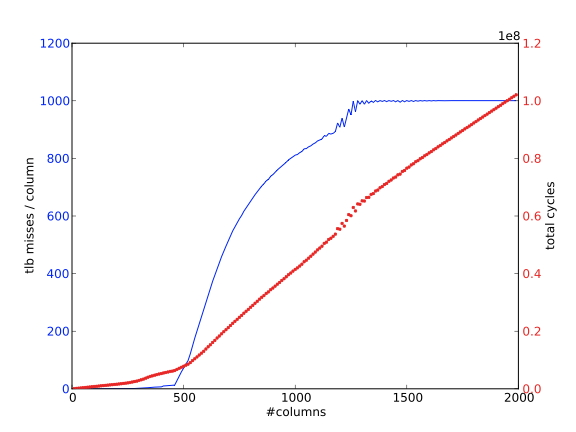
\includegraphics[scale=.35]{tlb_row}
\end{frame}

\begin{frame}[fragile]{TLB hits}
\small
\begin{verbatim}
#define INDEX(i,j,m,n) i+j*m
array = (double*) malloc(m*n*sizeof(double));
/* traversal #1 */
for (j=0; j<n; j++)
  for (i=0; i<m; i++)
    array[INDEX(i,j,m,n)] = array[INDEX(i,j,m,n)]+1;
\end{verbatim}
  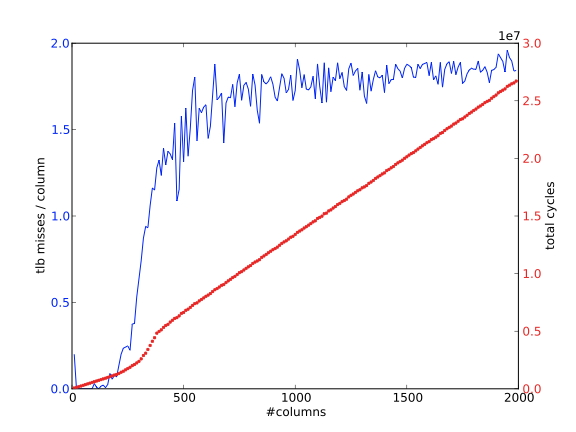
\includegraphics[scale=.35]{tlb_col}
\end{frame}

\begin{frame}{Little's Law}
  \begin{itemize}
  \item Item loaded from memory, processed, new item loaded in response
  \item But this can only happen after latency wait
  \item Items during latency are independent, therefore
    \[ \mathrm{Concurrency}=\mathrm{Bandwidth}\times \mathrm{Latency}. \]
  \end{itemize}
  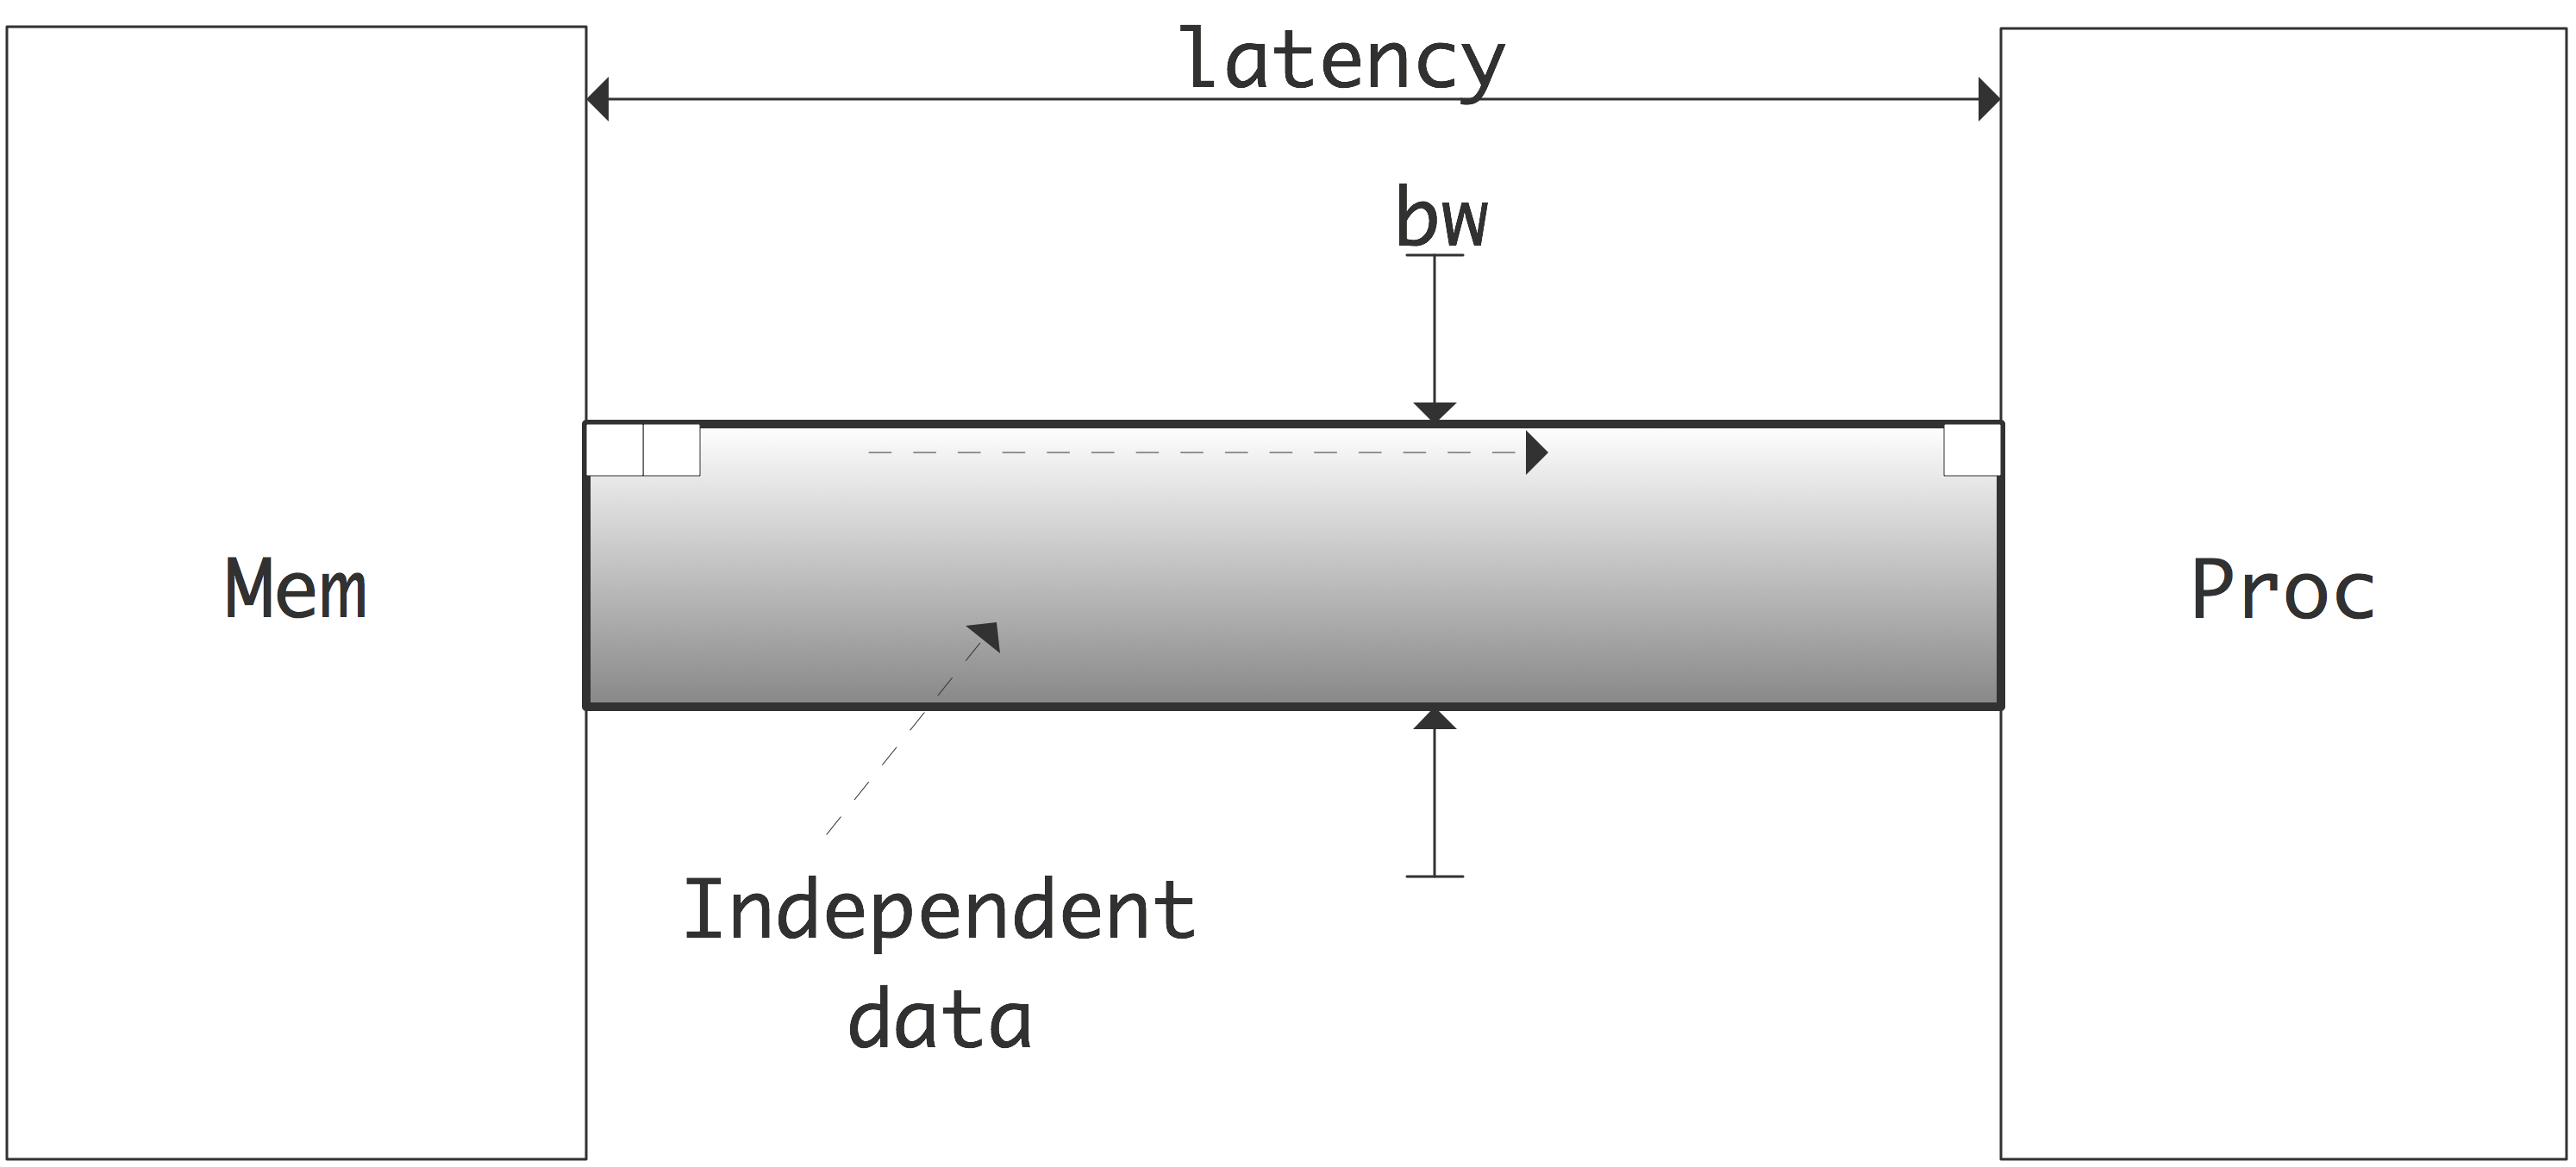
\includegraphics[scale=.1]{little}
\end{frame}

\Level 1 {Multicore issues}

\begin{frame}{Why multicore}
  Quest for higher performance:
  \begin{itemize}
  \item Two cores at half speed more energy-efficient than one at full speed.
  \item Not enough instruction parallelism for long pipelines
  \end{itemize}
  Multicore solution:
  \begin{itemize}
  \item More theoretical performance
  \item Burden for parallelism is now on the programmer
  \end{itemize}
\end{frame}

\begin{frame}{Multicore caches}
  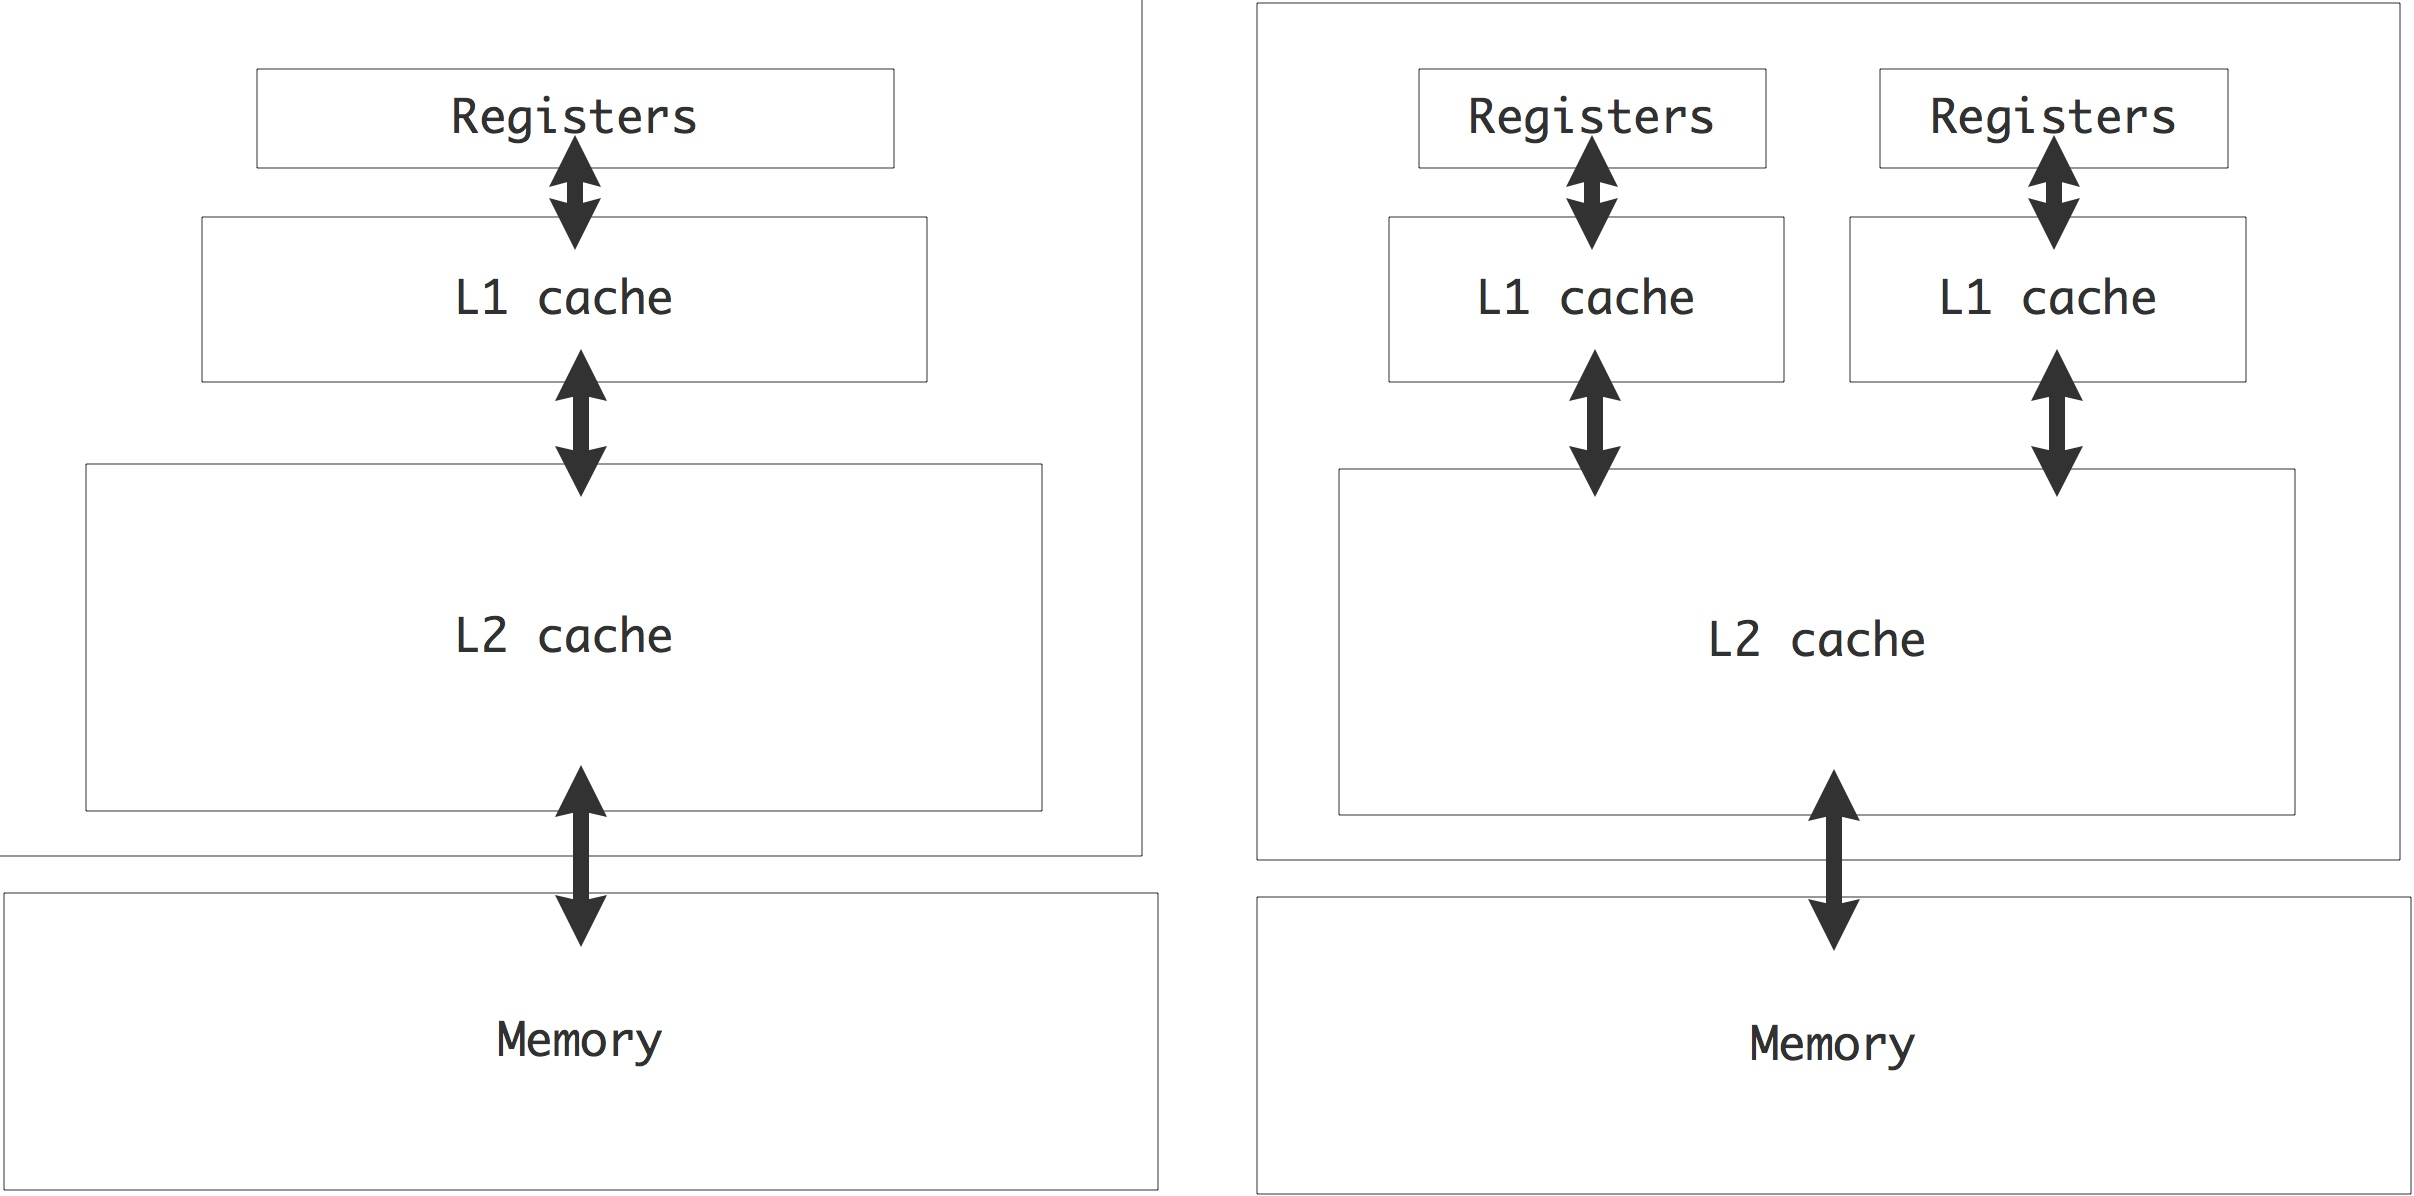
\includegraphics[scale=.12]{cache-hierarchy}
\end{frame}

\begin{frame}{Cache coherence}
\acf{MSI} coherence protocol:
\begin{description}
\item [Modified:] the cacheline has been modified
\item [Shared:] the line is present in at least one cache and is unmodified.
\item [Invalid:] the line is not present, or it
  is present but a copy in another cache has been modified.
\end{description}
\end{frame}

\begin{frame}[fragile]{Coherence issues}
  \begin{itemize}
  \item Coherence is automatic, so you don't have to worry about it\ldots
  \item \ldots except when it saps performance
  \item Beware false sharing\\
    writes to different elements of a cache line
  \end{itemize}
\end{frame}

\begin{frame}{Balance analysis}
  \begin{itemize}
  \item Sandy Bridge core can aborb 300 GB/s
  \item 4 DDR3/1600 channels provide 51 GB/s, difference has to come from reuse
  \item It gets worse: latency 80ns, bandwidth 51 GB/s, \\
    Little's law: parallelism 64 cache lines
  \item However, each core only has 10 line fill buffers,\\
    so we need 6--7 cores to provide the data for one core
  \item Power: cores are 72\%, uncore 17, DRAM~11.
  \item Core power goes 40\% to instruction handling, not arithmetic
  \item Time for a redesign of processors and programming; see my research presentation
  \end{itemize}
\end{frame}

\Level 1 {Programming strategies for performance}

\begin{frame}{How much performance is possible?}
  Performance limited by
  \begin{itemize}
  \item Processor peak performance: absolute limit
  \item Bandwidth: linear correlation with performance
  \end{itemize}
  \indexterm{Arithmetic intensity}: ratio of operations per transfer

  If AI high enough: processor-limited\\
  otherwise: bandwidth-limited
\end{frame}

\begin{frame}
  Performance depends on algorithm:

  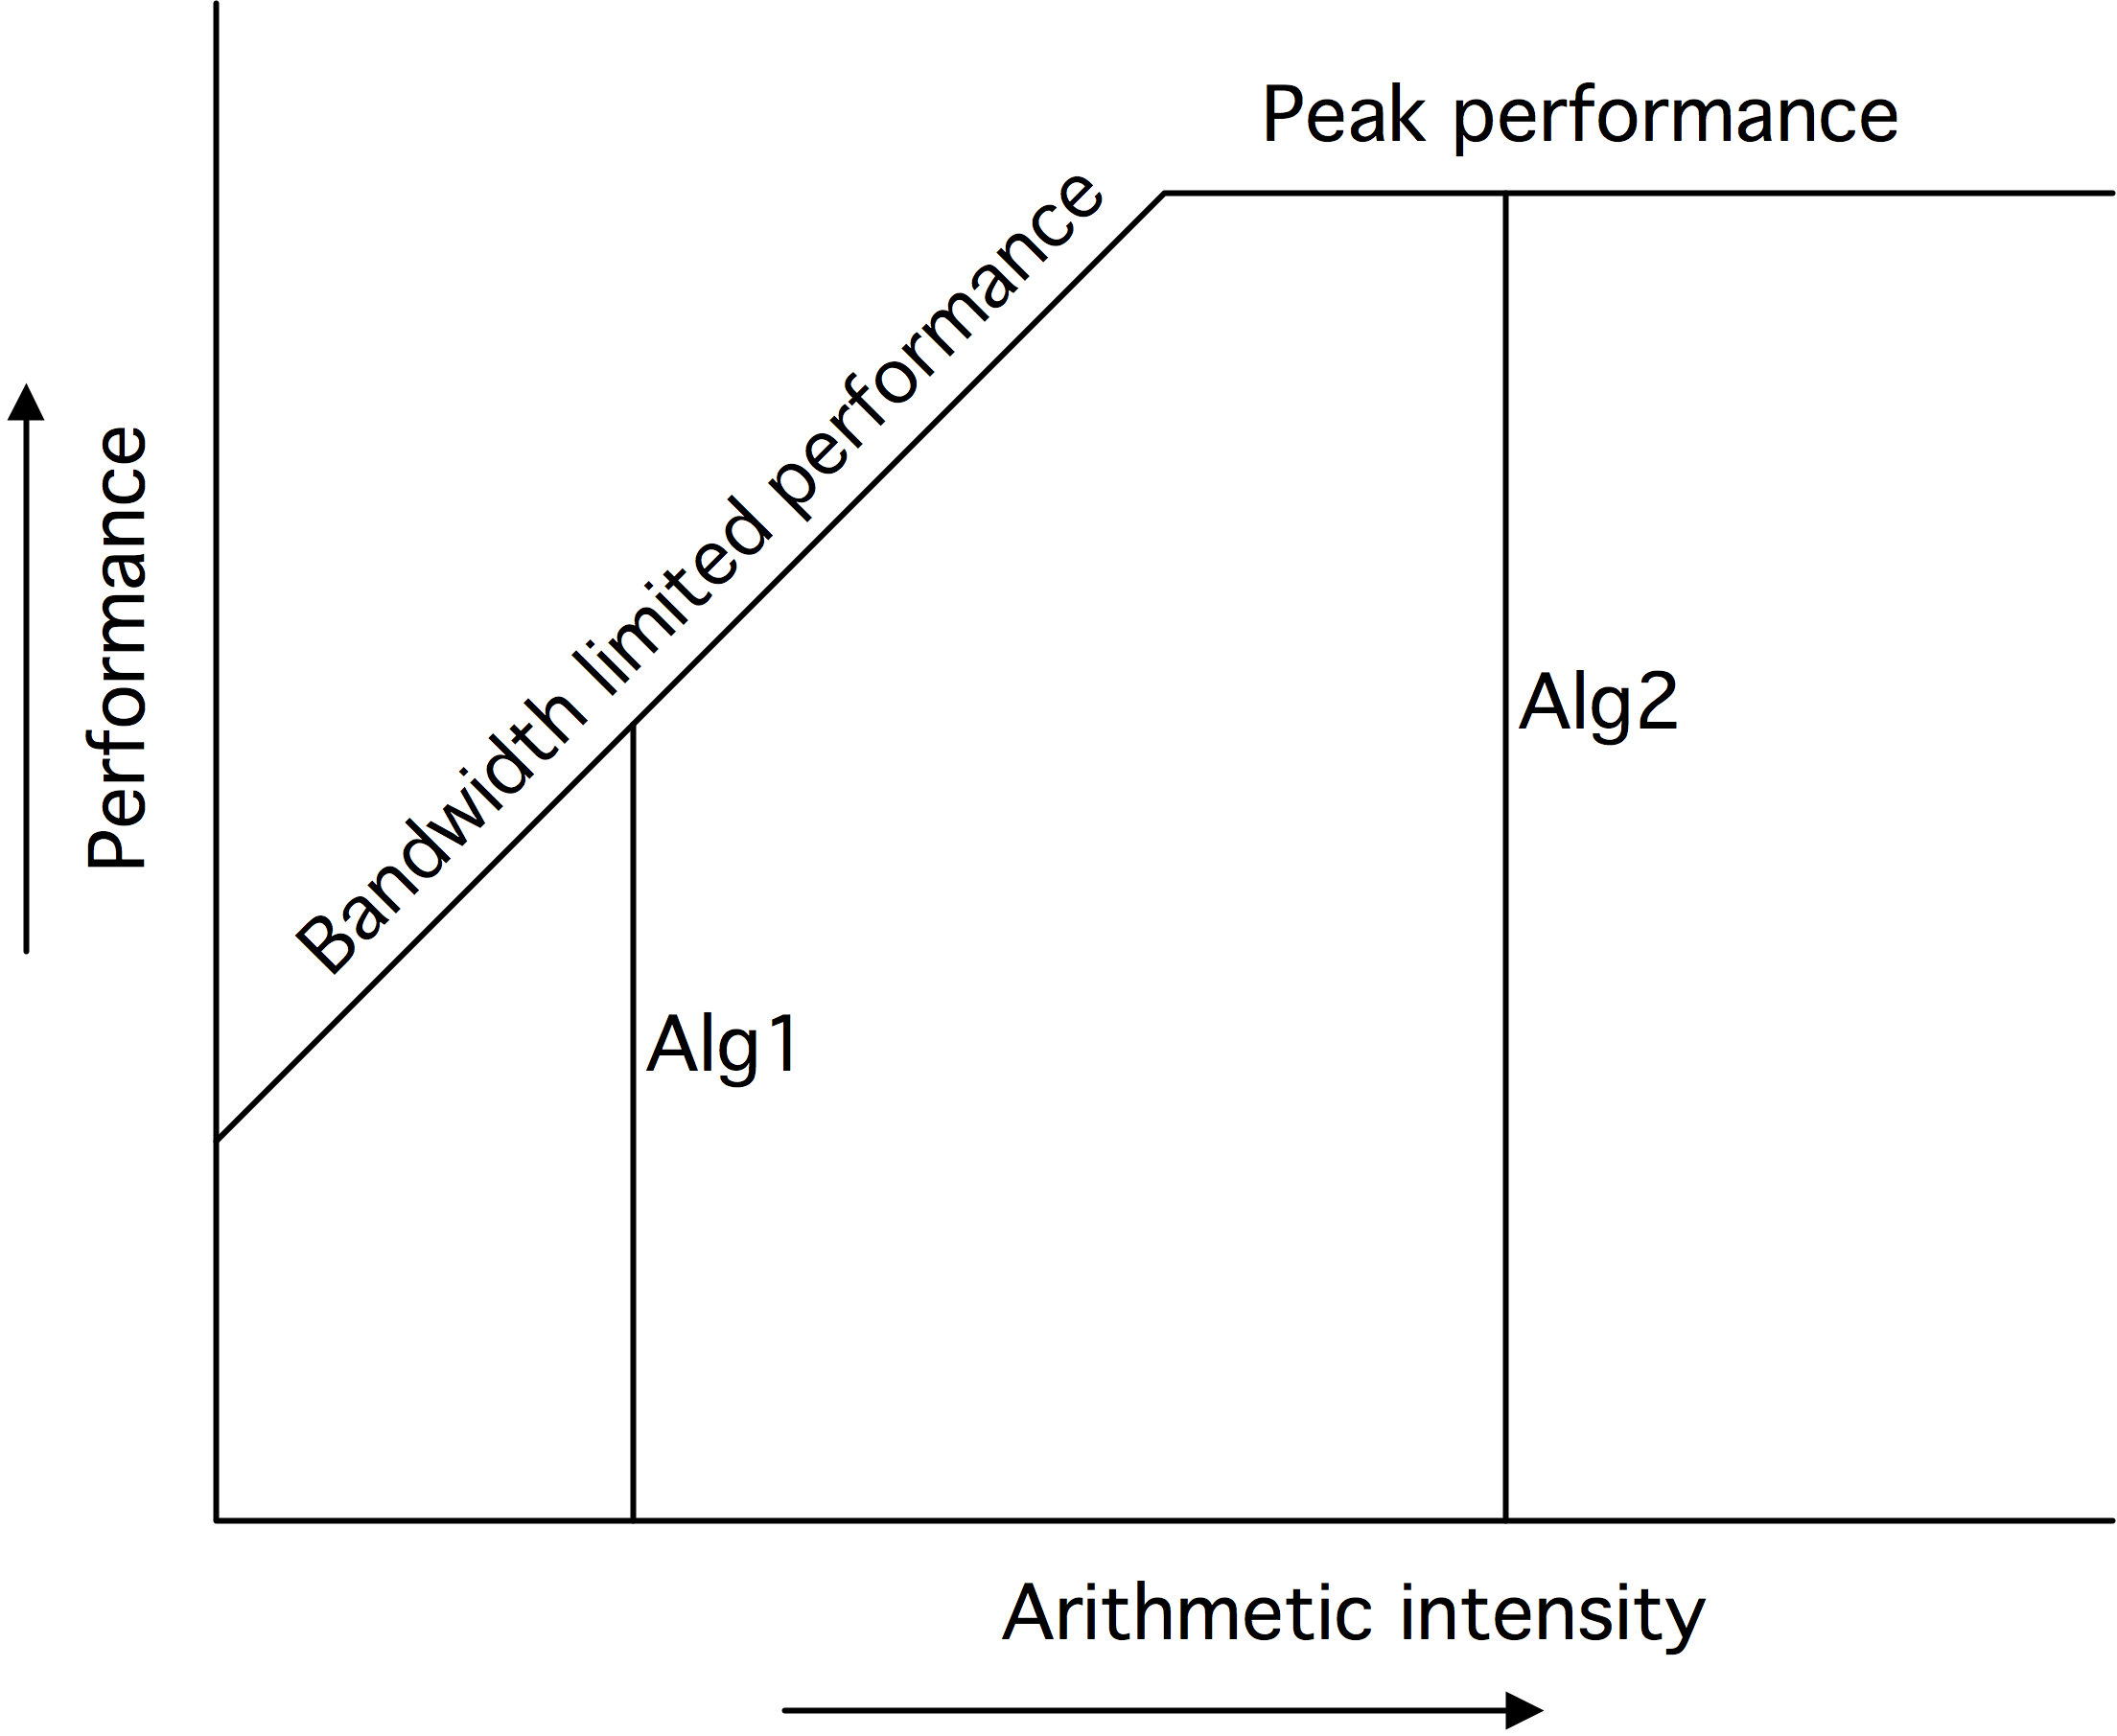
\includegraphics[scale=.1]{roofline1}
\end{frame}

\begin{frame}
  Insufficient utilization of functional units:

  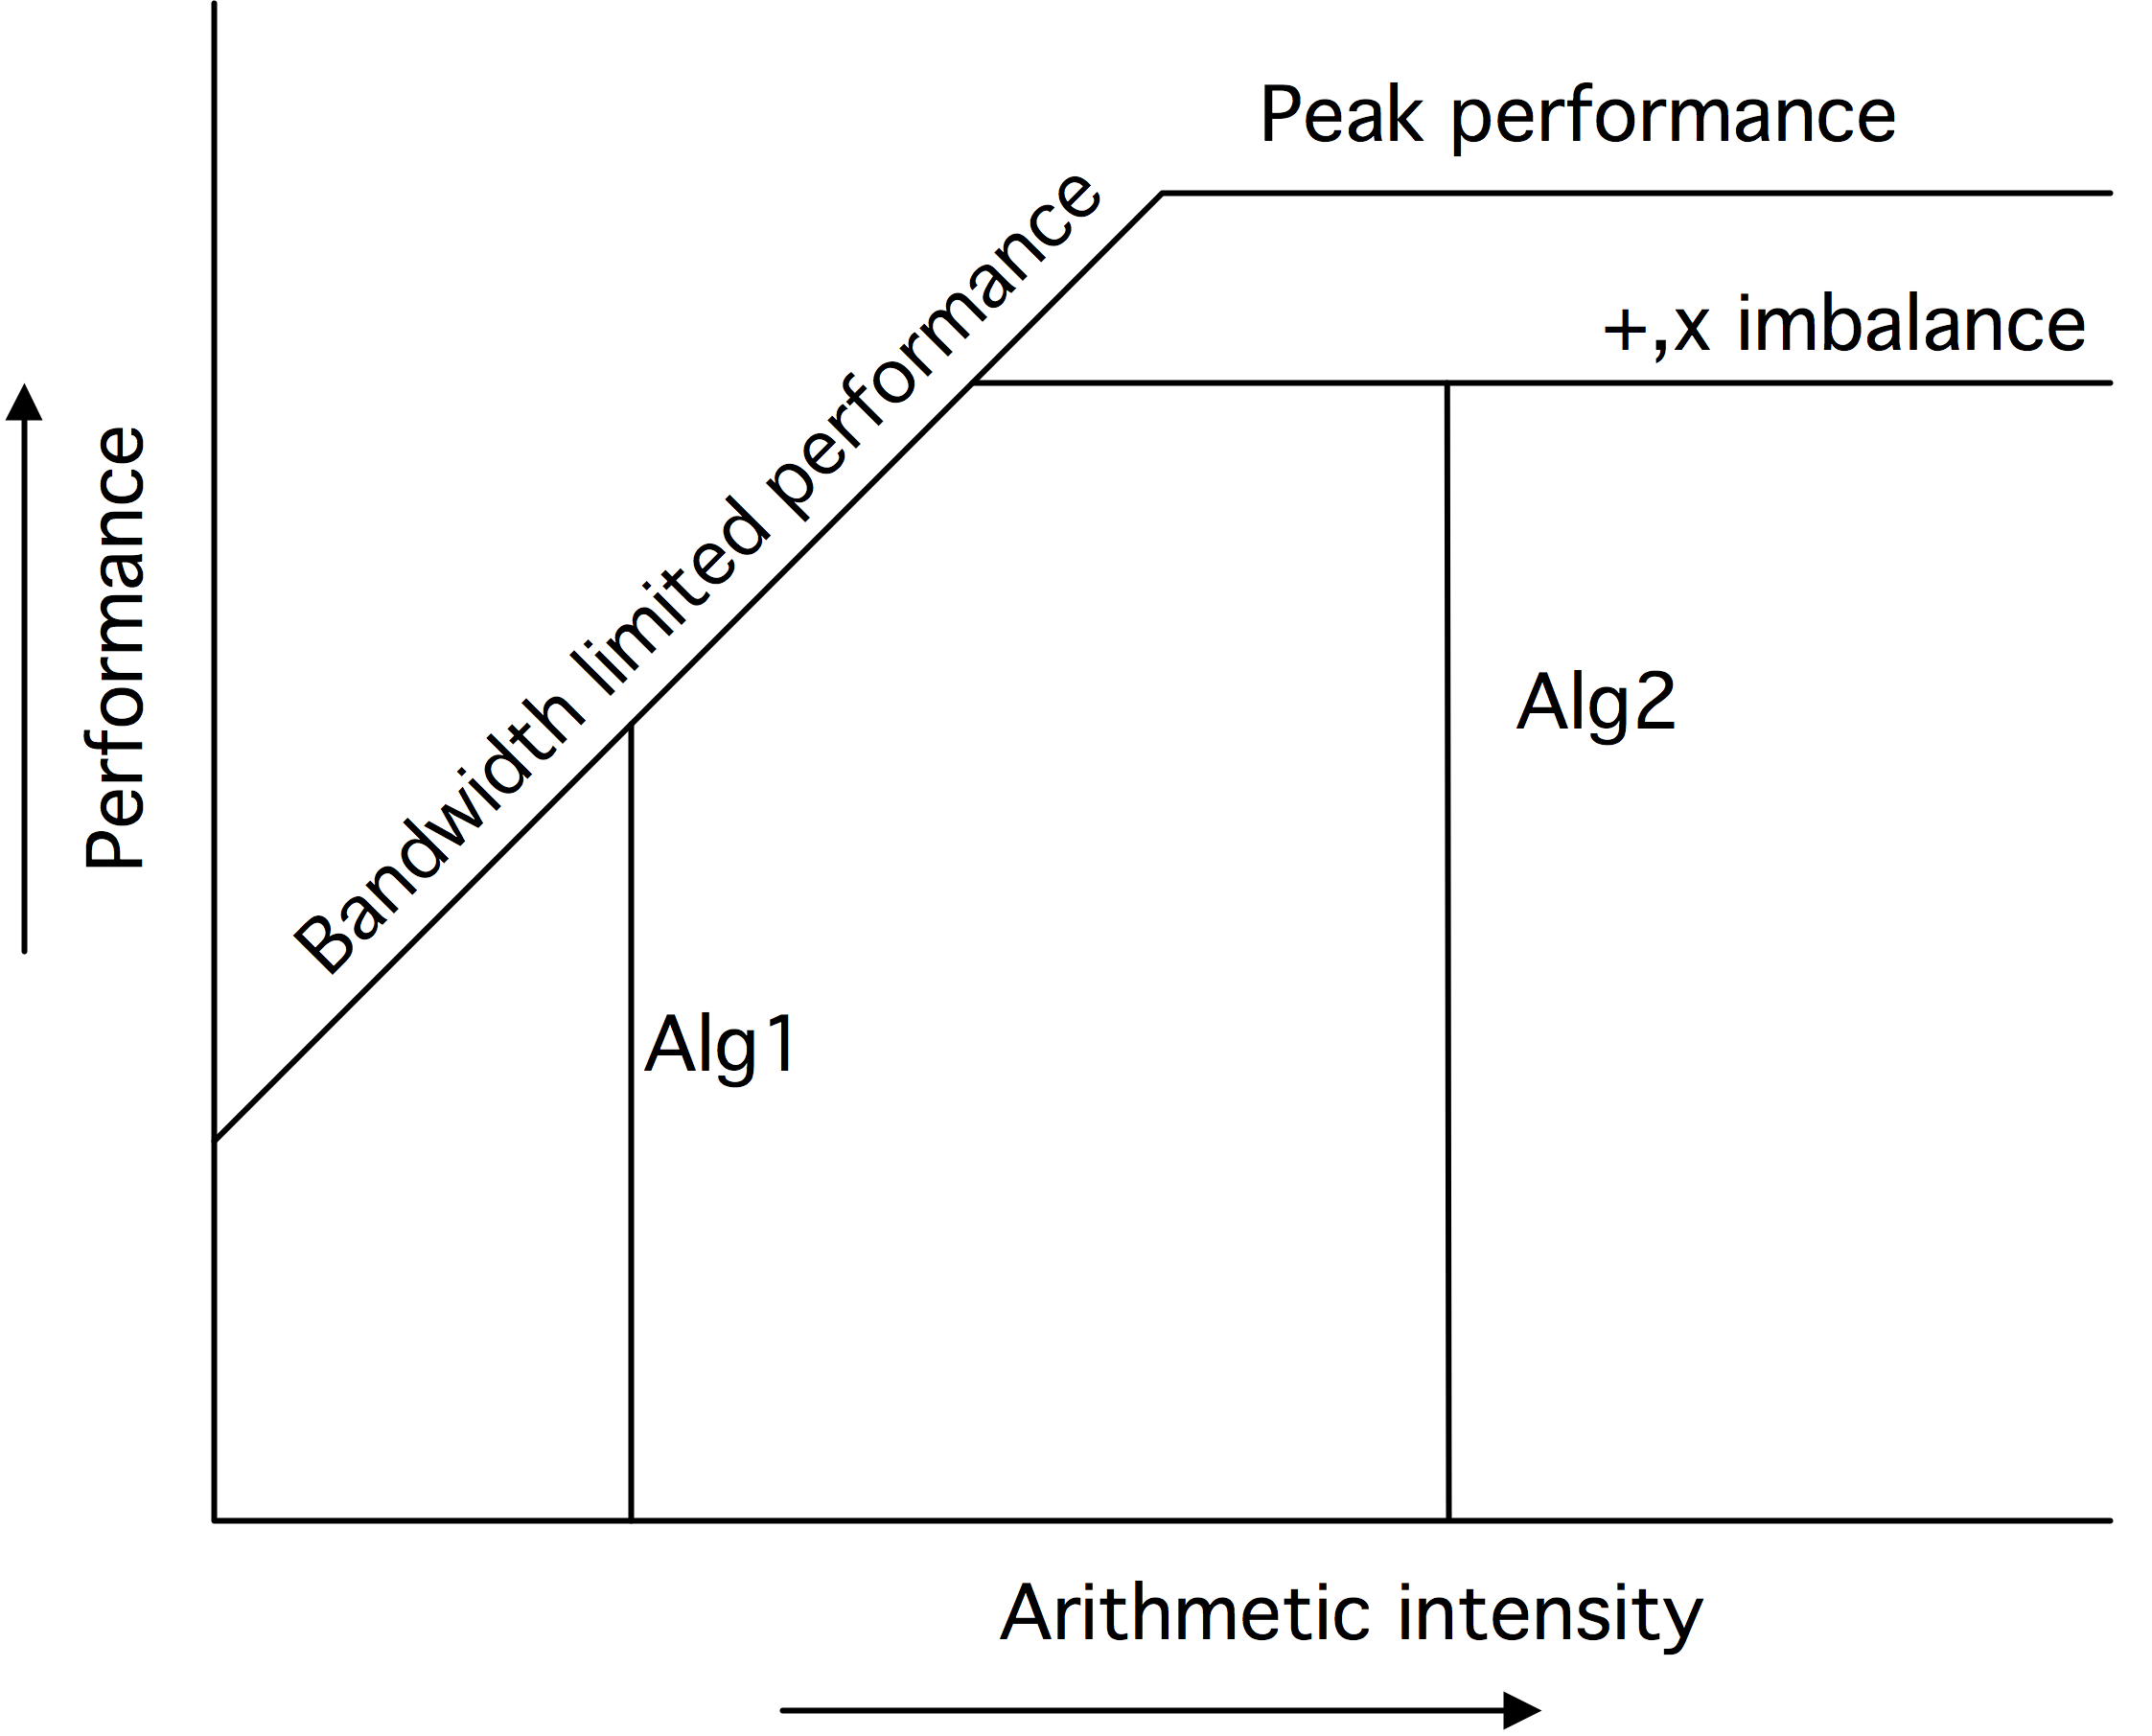
\includegraphics[scale=.1]{roofline2}
\end{frame}

\begin{frame}
  Imperfect data transfer:

  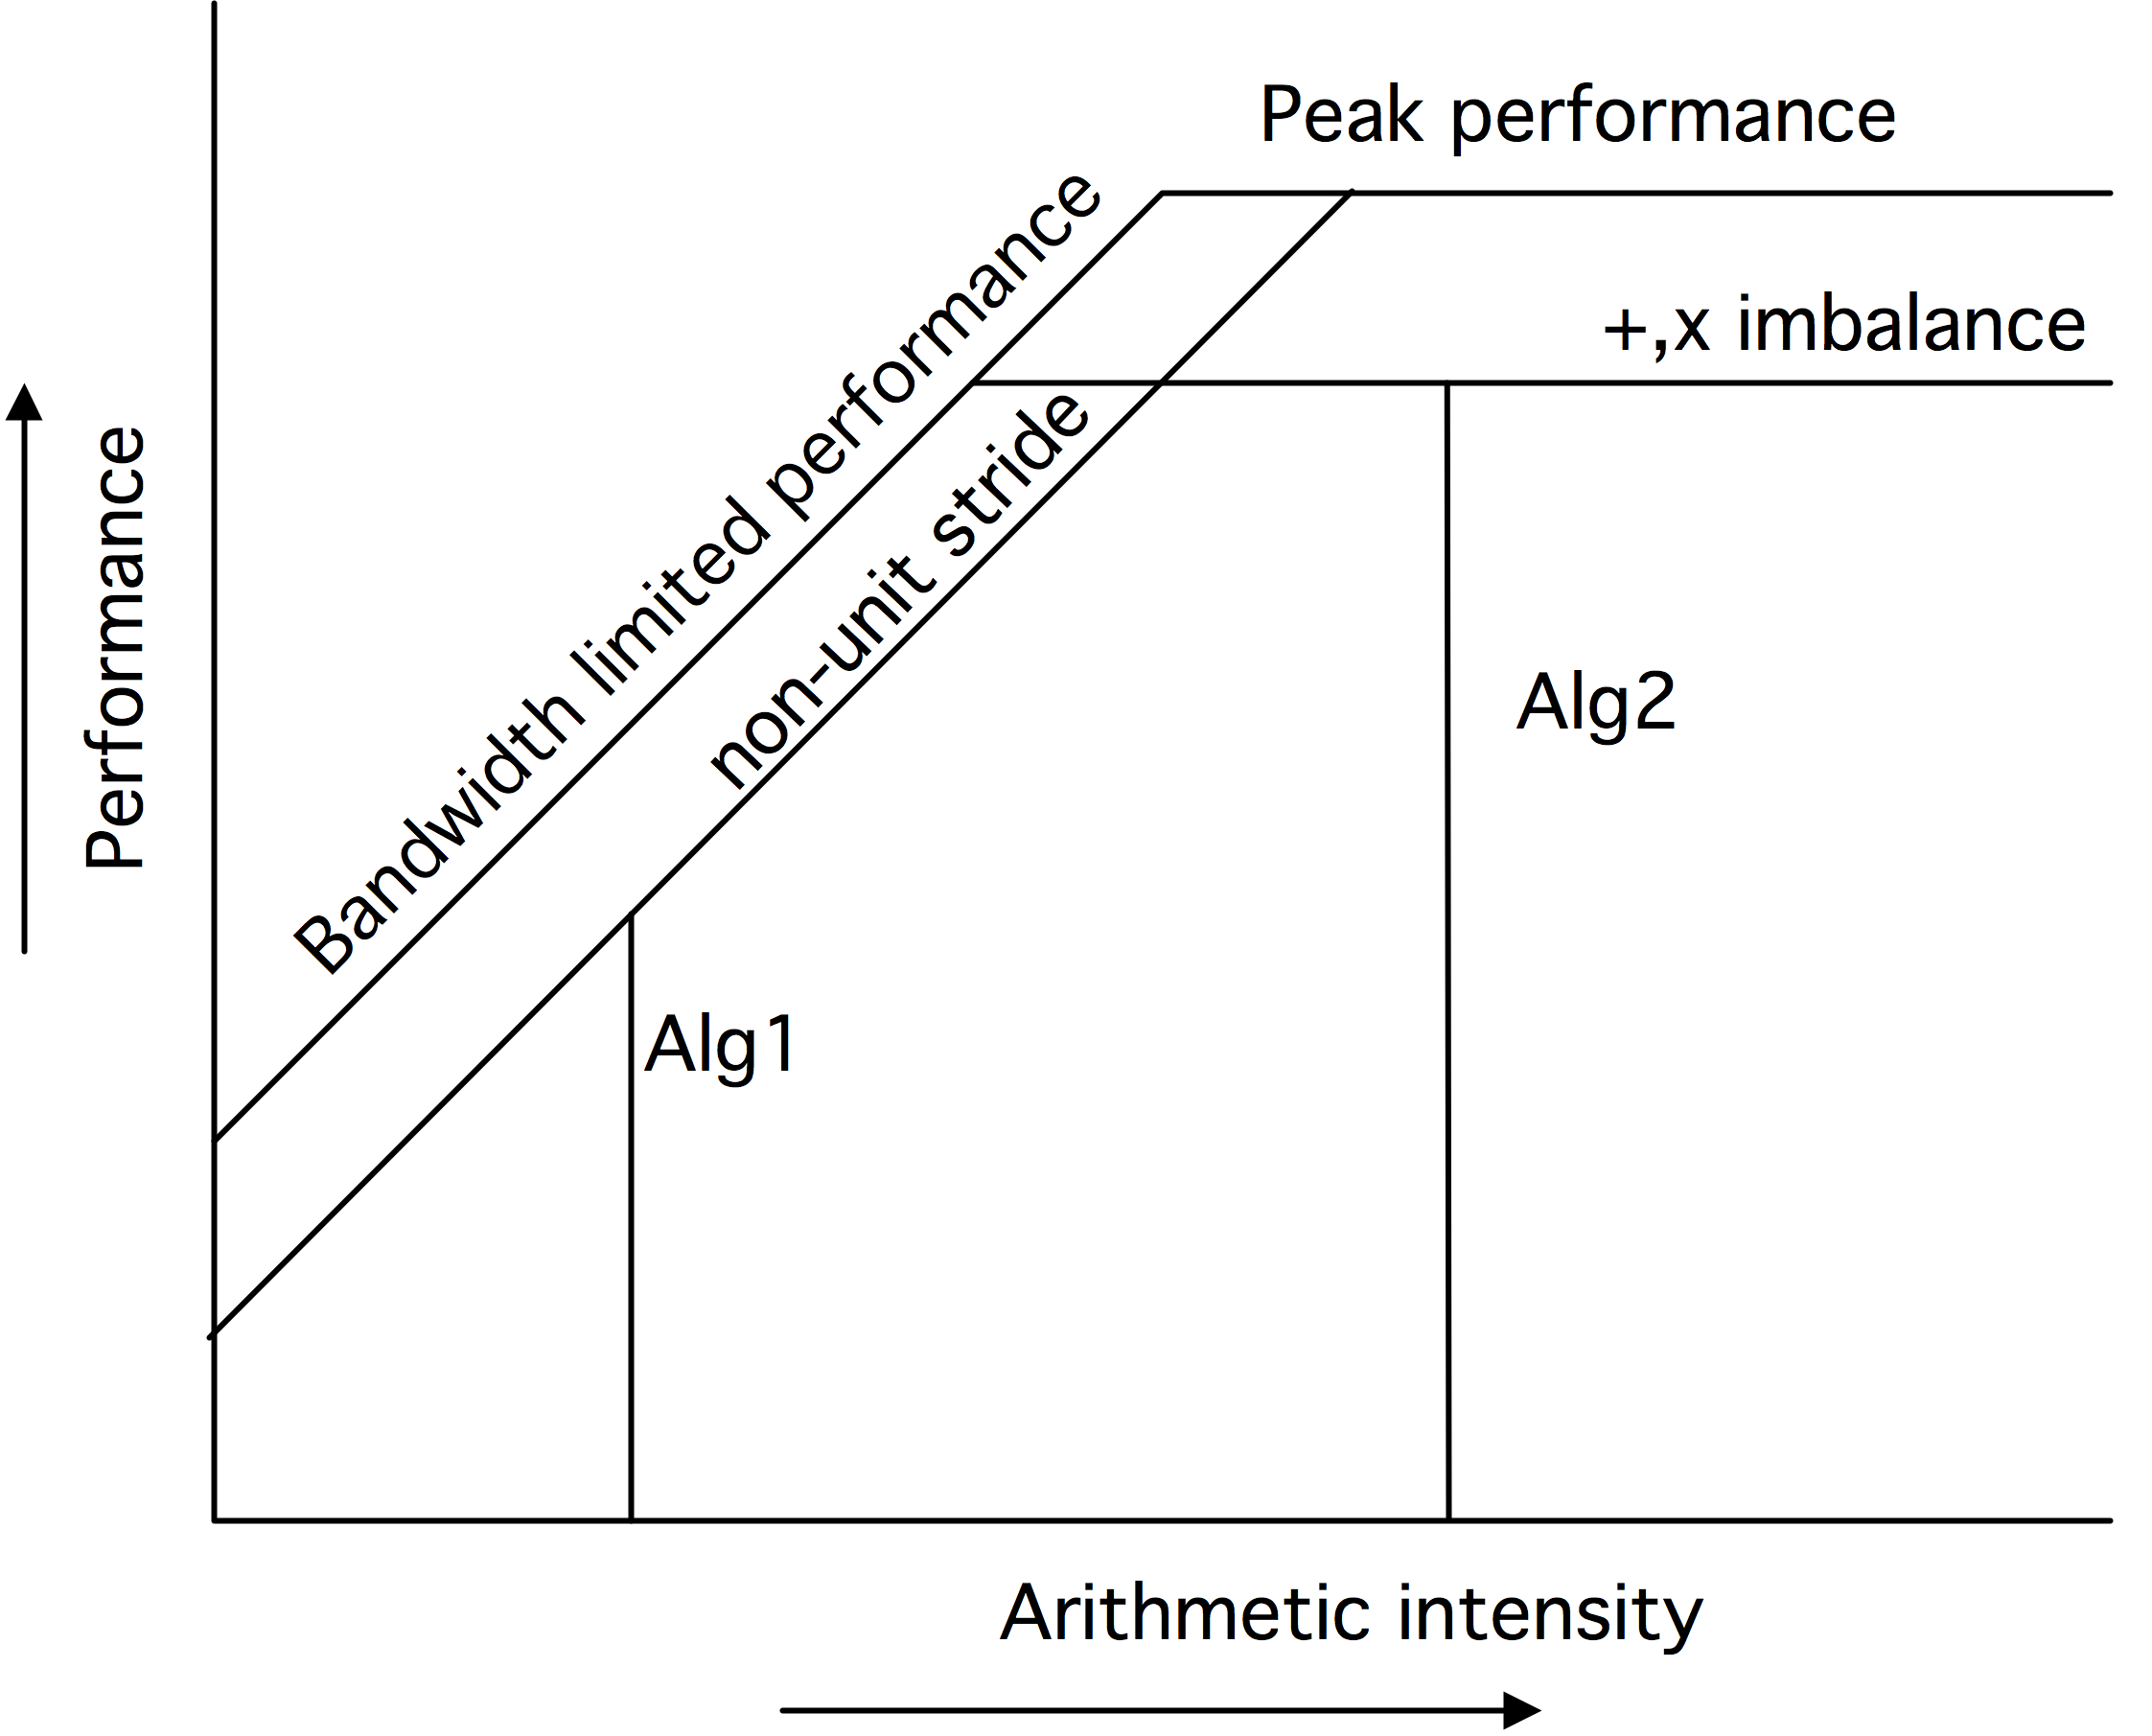
\includegraphics[scale=.1]{roofline3}
\end{frame}

\begin{frame}{Architecture aware programming}
  \begin{itemize}
  \item Cache size: block loops
  \item pipelining and vector instructions: expose streams of instructions
  \item reuse: restructure code (both loop merge and splitting, unroll
  \item TLB: don't jump all over memory
  \item associativity: watch out for powers of 2
  \end{itemize}
\end{frame}

\begin{frame}[fragile]{Loop blocking}
Multiple passes over data
\begin{verbatim}
for ( k< small bound )
  for ( i < N )
    x[i] = f( x[i], k, .... )
\end{verbatim}
Block to be cache contained
\begin{verbatim}
for ( ii < N; ii+= blocksize )
  for ( k< small bound )
    for ( i=ii; i<ii+blocksize; i++ )
      x[i] = f( x[i], k, .... )
\end{verbatim}
This requires independence of operations
\end{frame}

\begin{frame}{The ultimate in performance programming: DGEMM}
  Matrix-matrix product $C=A\cdot B$
  \[ \forall_i\forall_j\forall_k\colon c_{ij}\mathop{+=} a_{ik}b_{kj} \]
  \begin{itemize}
  \item Three independent loop $i,j,k$
  \item all three blocked $i',j',k'$
  \item Many loop permutations, blocking factors to choose
  \end{itemize}
\end{frame}

\begin{frame}[fragile]{DGEMM variant}
Inner products
\begin{verbatim}
for ( i )
  for ( j )
    for ( k )
      c[i,j] += a[i,k] * b[k,j]
\end{verbatim}
\end{frame}

\begin{frame}[fragile]{DGEMM variant}
Outer product: updates with low-rank columns-times-vector
\begin{verbatim}
for ( k )
  for ( i )
    for ( j )
      c[i,j] += a[i,k] * b[k,j]
\end{verbatim}
\end{frame}

\begin{frame}[fragile]{DGEMM variant}
Building up rows by linear combinations
\begin{verbatim}
for ( i )
  for ( k )
    for ( j )
      c[i,j] += a[i,k] * b[k,j]
\end{verbatim}
Exchanging $i,j$: building up columns
\end{frame}

\begin{frame}{Rank 1 updates}
  \[ C_{**} = \sum_k A_{*k}B_{k*} \]
  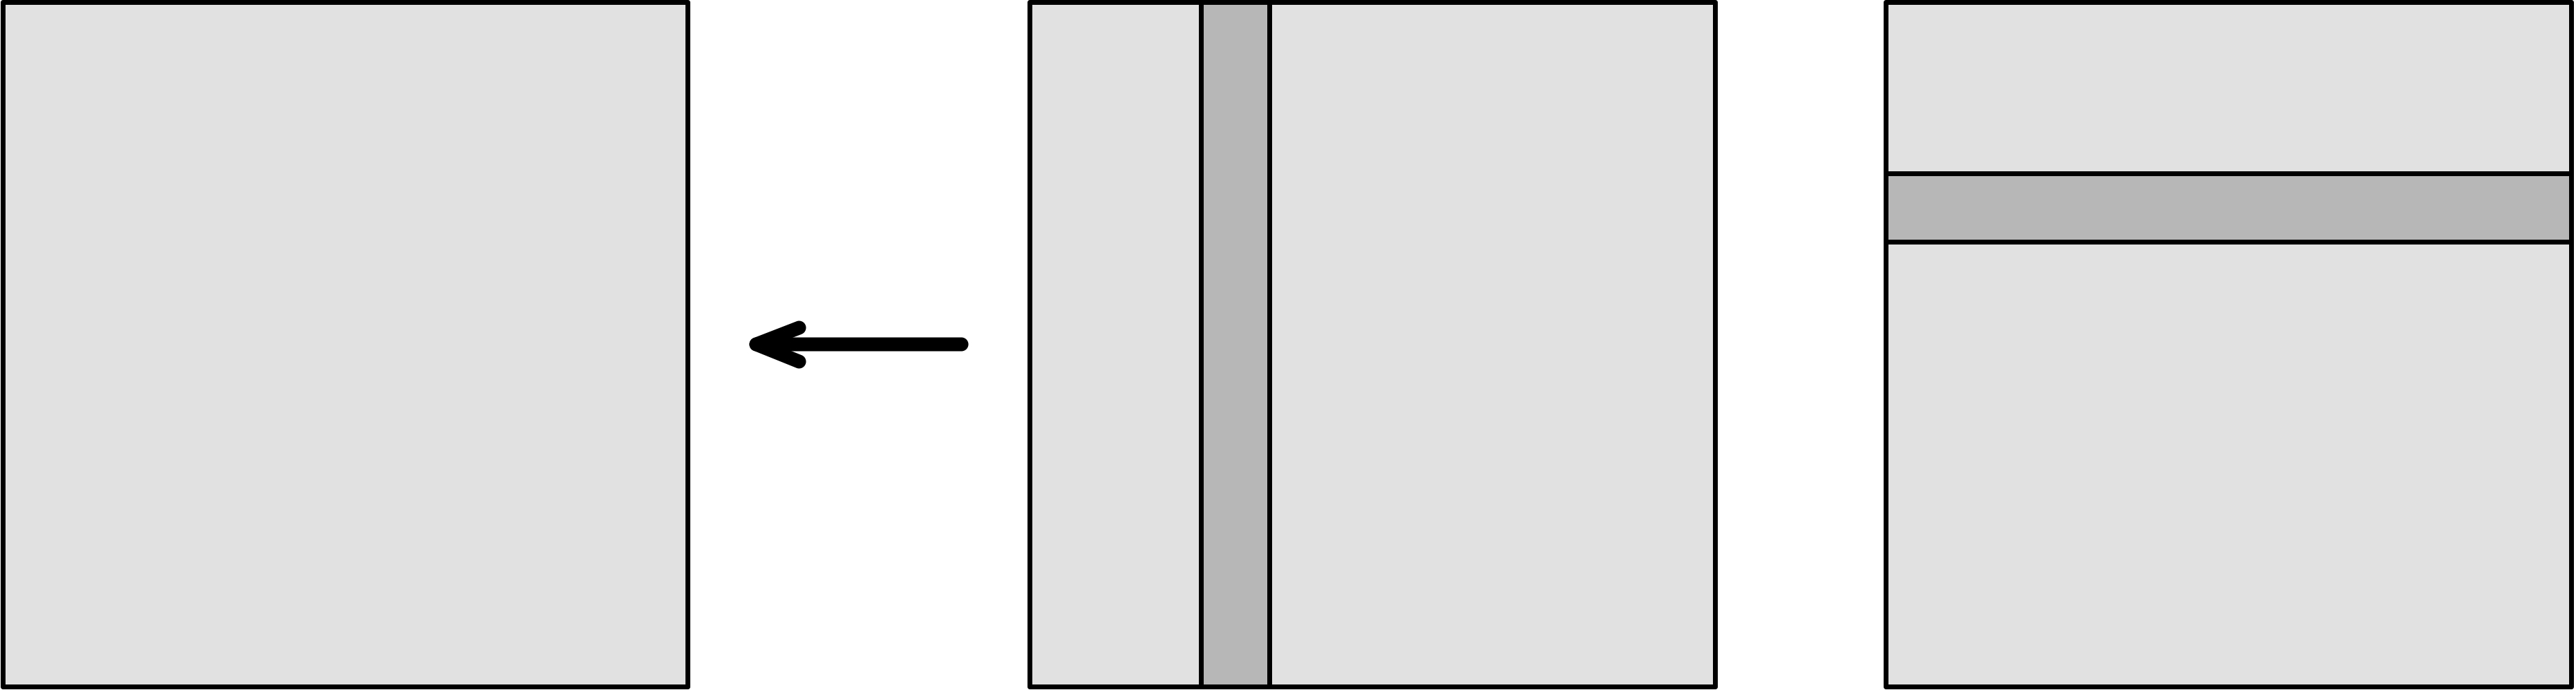
\includegraphics[scale=.07]{gotoblas1}
\end{frame}

\begin{frame}{Matrix-panel multiply}
  Block of $A$ times `sliver' of~$B$

  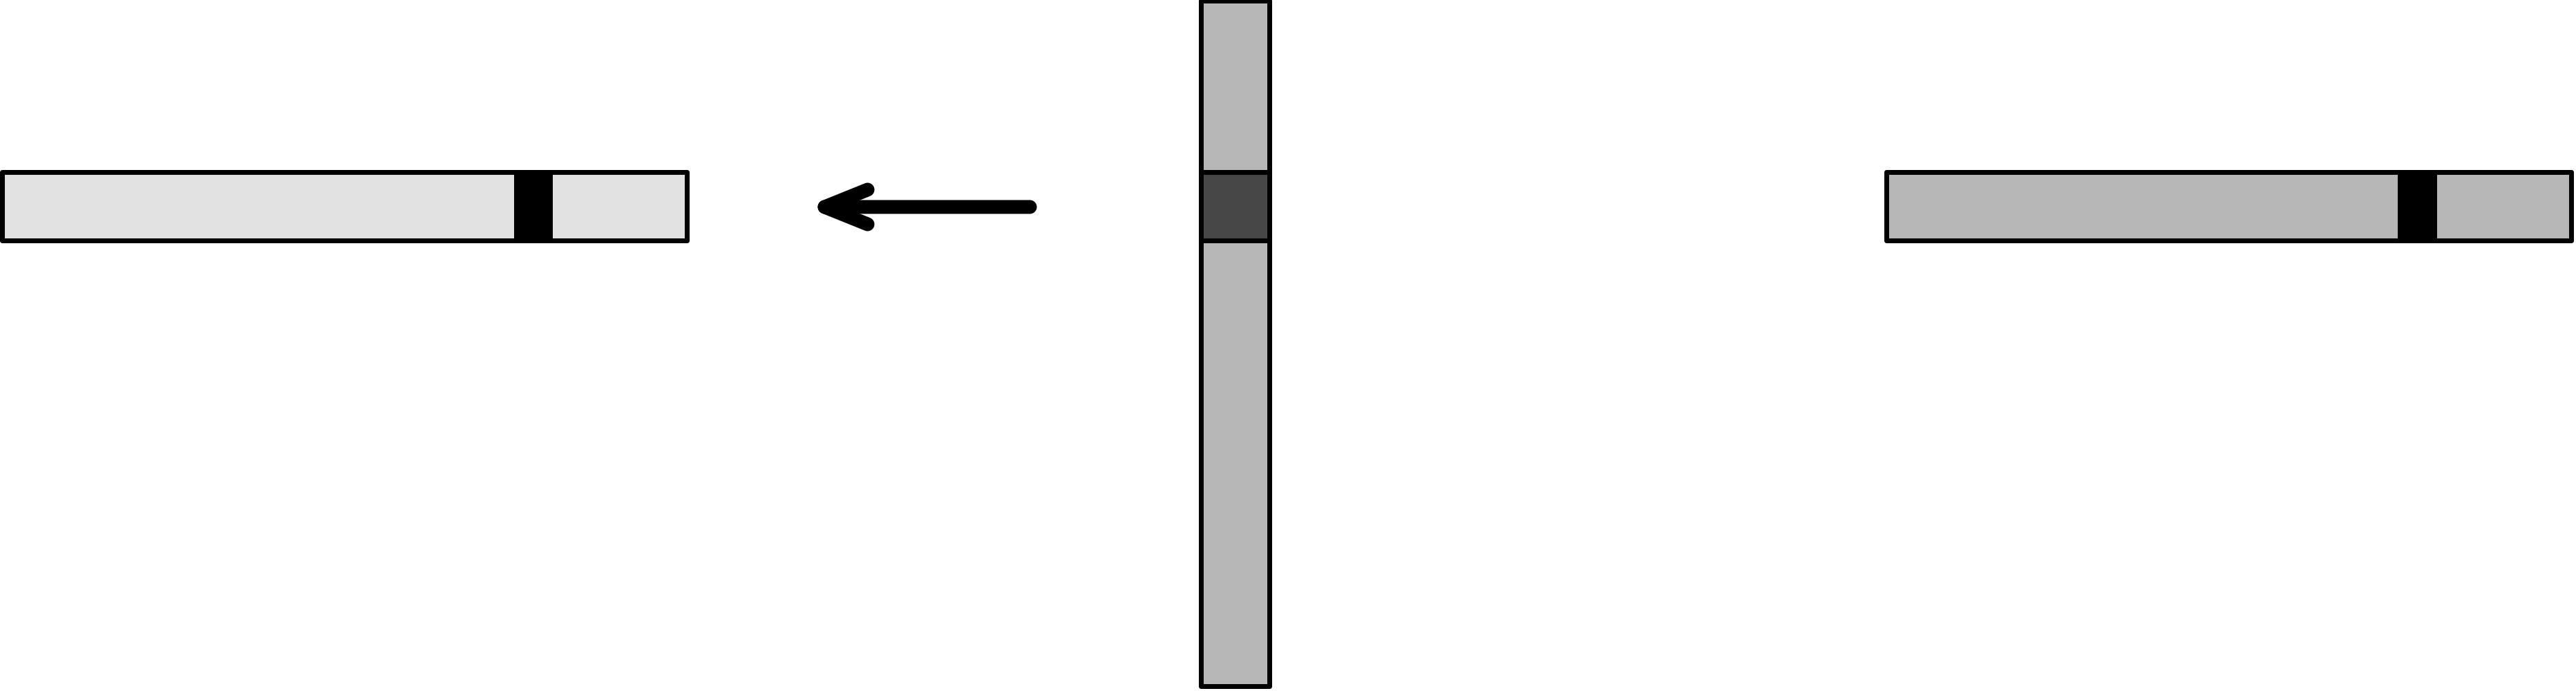
\includegraphics[scale=.08]{gotoblas2}  
\end{frame}

\begin{frame}[fragile]{Inner algorithm}
For inner $i$:
\begin{verbatim}
// compute C[i,*] :
for k:
   C[i,*] = A[i,k] * B[k,*]
\end{verbatim}
  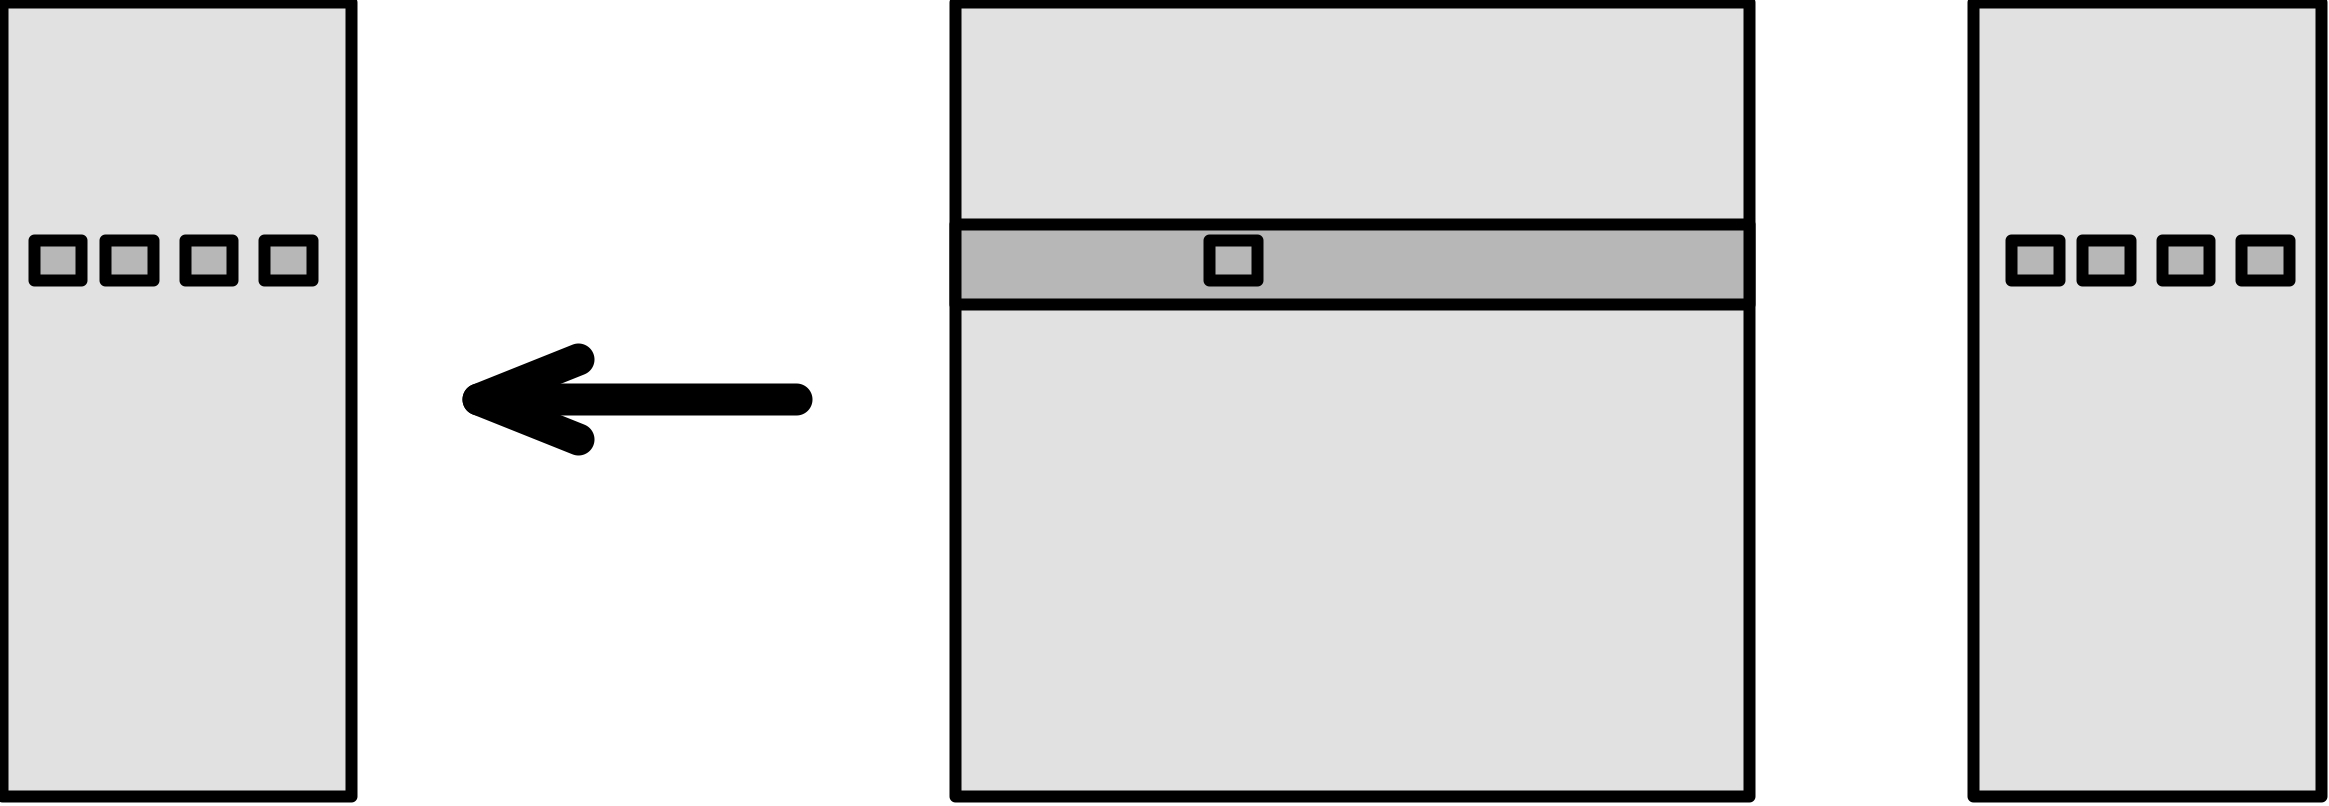
\includegraphics[scale=.1]{gotoblas3}
\end{frame}

\begin{frame}[fragile]{Tuning}
For inner $i$:
\begin{verbatim}
// compute C[i,*] :
for k:
   C[i,*] += A[i,k] * B[k,*]
\end{verbatim}
\begin{itemize}
\item \verb+C[i,*]+ stays in register
\item \verb+A[i,k]+ and \verb+B[k,*]+ stream from L1
\item blocksize of $A$ for L2 size
\item $A$ stored by rows to prevent TLB problems
\end{itemize}
\end{frame}

\begin{frame}{Cache-oblivious programming}
Observation: recursive subdivision will ultimately
make a problem small / well-behaved enough
  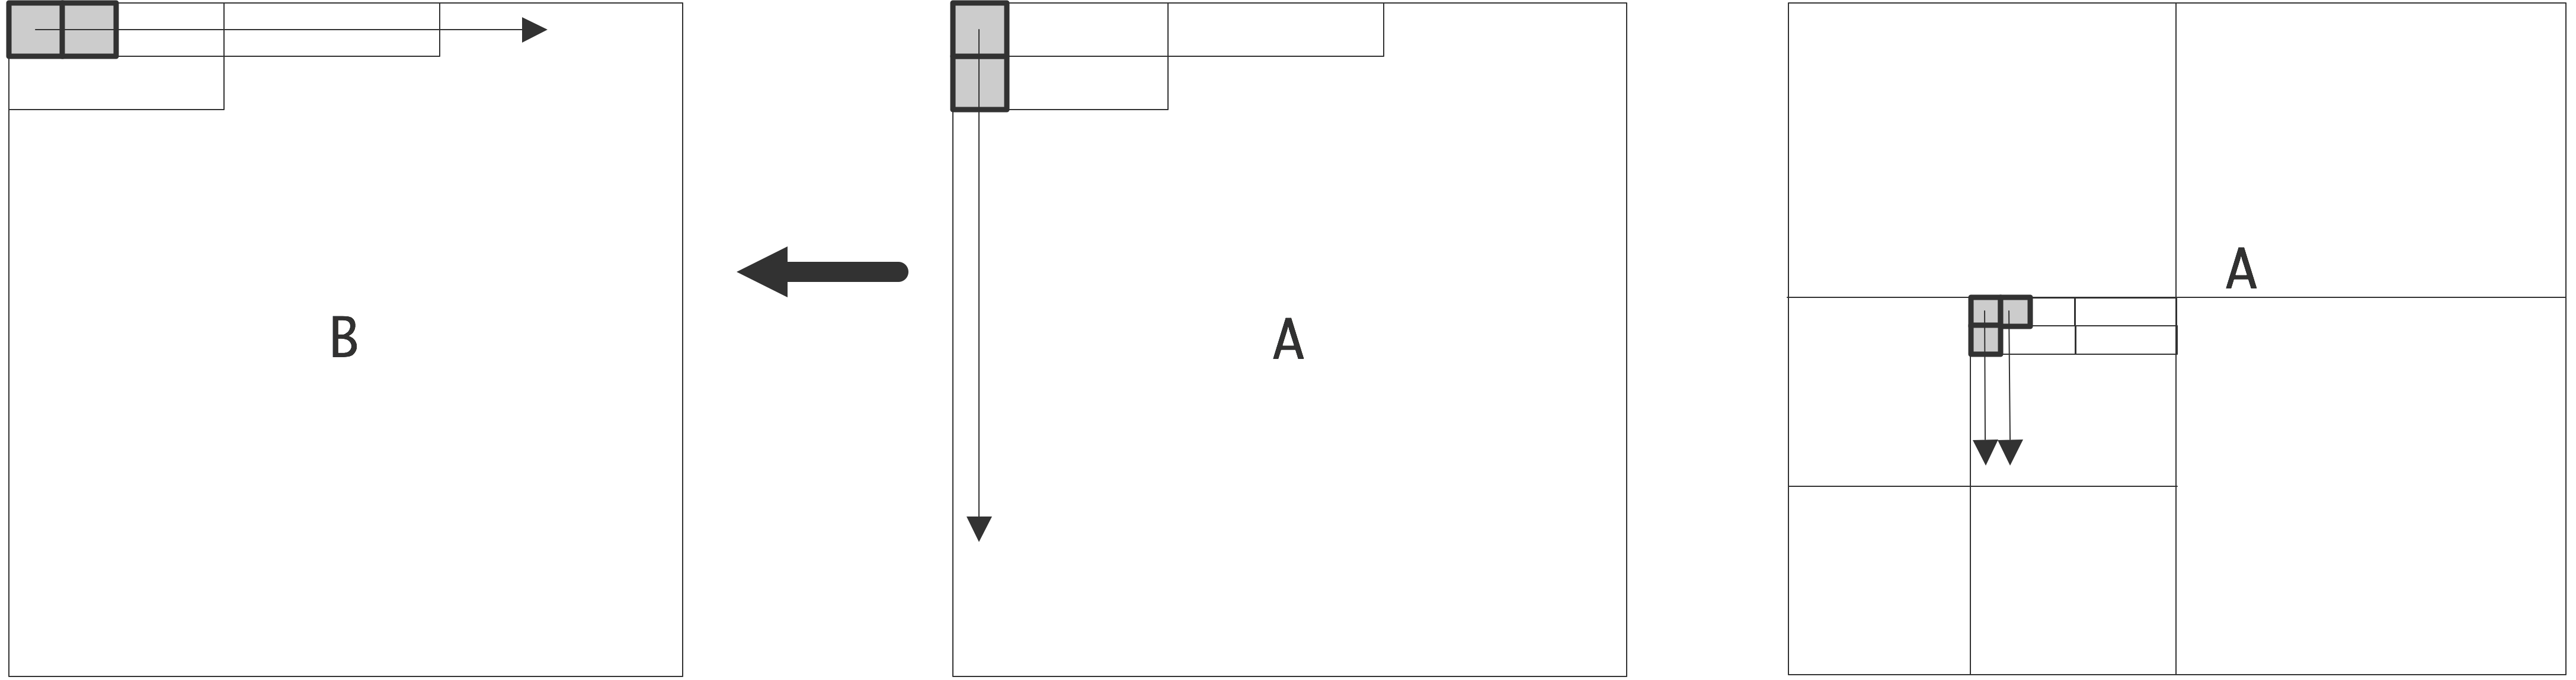
\includegraphics[scale=.08]{oblivious1}
\end{frame}

\begin{frame}{Cache-oblivious matrix-matrix multiply}
  \[ 
  \begin{pmatrix}
    C_{11}&C_{12}\\ C_{21}&C_{22}
  \end{pmatrix}
  =
  \begin{pmatrix}
    A_{11}&A_{12}\\ A_{21}&A_{22}
  \end{pmatrix}
  \begin{pmatrix}
    B_{11}&B_{12}\\ B_{21}&B_{22}
  \end{pmatrix}
  \]
  with $C_{11}=A_{11}B_{11}+A_{12}B_{21}$

  Recursive approach will be cache contained.\\
  Not as high performance as being cache-aware\ldots  
\end{frame}

\Level 1 {The power question}

\begin{frame}{Dennard scaling}
Scale down feature size by~$s$:
\[
\begin{array}{|l|c|}\hline
\hbox{Feature size}&\sim s\\
\hbox{Voltage}&\sim s\\
\hbox{Current}&\sim s \\ 
\hbox{Frequency}&\sim s\inv\\
\hline
\end{array}
\]  
Miracle conclusion:
\[ \hbox{Power} = V\cdot I \sim s^2; \hbox{Power density}\sim 1 \]
Everything gets better, cooling problem stays the same

Opportunity for more components, higher frequency
\end{frame}

\begin{frame}{Dynamic power}
\begin{equation}
\begin{array}{|l|l|} \hline
\hbox{Charge}&q=CV\\
\hbox{Work}&W=qV=CV^2\\
\hbox{Power}&W/\hbox{time}=WF=CV^2F \\ \hline
\end{array}
\label{eq:power}
\end{equation}  
Two cores at half frequency:
\[ \left.
\begin{array}{c}
C_{\mathrm{multi}} = 2C\\
F_{\mathrm{multi}} = F/2\\
V_{\mathrm{multi}} = V/2\\
\end{array}\right\} \Rightarrow
P_{\mathrm{multi}} = P/4.
\]
Same computation, less power
\end{frame}

